\documentclass[a4paper]{article}

\usepackage[english]{babel}
\usepackage[utf8]{inputenc}
\usepackage{amsmath}
\usepackage{graphicx}
\usepackage{subcaption}
\usepackage[numbered]{bookmark}
\usepackage[colorinlistoftodos]{todonotes}
\usepackage{algorithm}
\usepackage{algpseudocode}
\usepackage{pifont}
\usepackage{tikz}
\usepackage{pgfplots}
\usepackage{bm}
\usepackage{placeins}
\usetikzlibrary{arrows}
\usetikzlibrary{external}\tikzexternalize[prefix=figs/]

\DeclareGraphicsExtensions{.eps,.pdf,.png,.tikz}
\graphicspath{{figs/}}

\title{Coherent Detection Systems for Data Centers}

\author{JKP}

\date{\today}

\begin{document}
\maketitle

\section{Transmitter}
\subsection{Intensity Noise}
Intensity noise is modeled as an AWGN added to the optical power at the transmitter.

The value of the relative intensity noise (RIN) is defined as the ratio between the noise power divide by the noise bandwidth and the signal power \cite{agilent-RIN-measurement}: 
\begin{equation}
RIN = \frac{P_{noise}}{B_{noise}P_{signal}}
\end{equation}

Hence, the \textbf{one-sided RIN PSD} and \textbf{RIN variance} at a certain instant are given by
\begin{align}
& S_{RIN}(t) = RIN\cdot P(t)^2 \\
& \sigma^2_{RIN}(t) = S_{RIN}(t)\frac{f_{s, sim}}{2}
\end{align}
where $f_{s, sim}$ is the sampling frequency to simulate continuous time. Obviously, the variance as defined here only make sense in simulations. Since the intensity noise is assumed to be white, it'd have infinite variance.

Output optical power $P(t)$ is given by
\begin{equation}
P(t) = P_s(t) + w_{RIN}(t)
\end{equation}
where $P_s(t)$ is the signal-only optical power (after modulator frequency response and extinction ratio), and $w_{RIN}(t)\sim\mathcal{N}(0, \sigma^2_{RIN}(t))$.

\subsection{Modulator Bandwidth Limitations}

\subsubsection{Mach-Zenhder modulator}
\cite{Barros2009, Ho2005}

Limited by loss and velocity mismatch

\begin{equation}
H_{mod}(f) = \frac{1-e^{-\alpha(f)L+j2\pi fd_{12}L}}{\alpha(f)L-j2\pi fd_{12}L}
\end{equation}
where $\alpha(f)$ is the frequency-dependent loss, $d_{12}$ is the velocity mismatch between the optical and electrical waveguides, and $L$ is the interaction length.

\begin{equation}
d_{12} = \frac{n_m-n_r}{c}
\end{equation}
where $n_r \approx 2.15$ is the refractive index of the coplanar waveguide for TM input light. If $n_m$ is only $95\%$ of $n_r$ a significant reduction in bandwidth may occur due to velocity mismatch \cite{Ho2005}.

\subsubsection{Modulator limited by parasitics}
This modulator is modeled as a critically damped second-order system. This is based on the assumption that parasitics capacitances and inductances are the limiting factor in the bandwidth of these devices.

Second-order system with unit damping:
\begin{equation}
H_{mod}(f) =  \frac{1}{1 + 2jf/f_c - (f/f_c)^2}
\end{equation}

The modulator bandwidth is related to $f_c$ by
\begin{equation}
f_{3dB} = \sqrt{\sqrt{2}-1}f_c = 0.64359f_c
\end{equation}

Group delay:
\begin{equation}
\Delta\tau_g = \frac{2}{2\pi f_c}
\end{equation}

\section{Fiber Propagation}
\subsection{Chromatic Dispersion}
\begin{equation} \label{eq:Hdisp}
H(f; L) = \frac{E(f; L)}{E(f, 0)} = e^{-1/2j\beta_2(2\pi f)^2L}
\end{equation}
where $H(f; L)$ is fiber frequency response due to dispersion after $L$ meters, and $\beta_2 = -\frac{D(\lambda)\lambda^2}{2\pi c}$. 

Fiber attenuation can be included with the factor $e^{-\frac{1}{2}\frac{att(\lambda)L}{10^4}}$, where $att(\lambda)$ is the fiber attenuation at wavelength $\lambda$ in dB/km.

For SMF28 the fiber dispersion is specified in terms of the zero-dispersion ($\lambda_0$) wavelength and the dispersion slope ($S_0$):
\begin{equation}
D(\lambda) = \frac{S_0}{4}\bigg(\lambda - \frac{\lambda_0^4}{\lambda^3}\bigg), 1200~\text{nm} < \lambda < 1600~\text{nm}
\end{equation}
where $\lambda_0 = 1310$ nm and $S_0 = 0.092$ ps/nm.

\section{OFDM}

\subsection{Symbol Rate and Sampling Rate}

We define an OFDM signal with $N_c$ orthogonal subcarriers, from which $N_c - N_u$ subcarriers are used for oversampling, leaving $N_u$ subcarriers to transmit date. Hence, the oversampling rate is defined as $r_{os} = \frac{N_c}{N_u}$. 

Different variations of OFDM may not use all the $N_u$ subcarriers available. A few examples are the case of when Hermitian symmetry is enforced to produce a real signal, or when half of the subcarriers are set to zero to produce a single-side band (SSB) signal, or when all the even subcarriers are not modulated to allow asymmetric clipping in asymmetrically clipped (ACO)-OFDM. This loss in spectral efficiency will be characterized by a factor $p$. Note that the definition of $N_u$ is different from the one used in the ``Multicarrier'' paper, where $N_u$ denoted the number of ``used'' subcarriers i.e., subcarriers not set to zero. 

Given a certain bit rate $R_b$, the spacing between each subcarrier is given by
\begin{equation} \label{eq:ofdm-subcarrier-spacing}
\Delta f = p\frac{R_b}{N_u\log_2 CS},
\end{equation}
where $CS$ is the nominal or average constellation size, and $p$ is the factor that accounts for the loss of spectral efficiency. For instance, $p = 2$ when Hermitian symmetry is enforced or when the negative subcarriers are set to zero in the case of SSB-OFDM. In the case of ACO-OFDM, $p = 4$ since in addition to Hermitian symmetry, all the even subcarriers are set to zero. 

Fig.~\ref{fig:ofdm-spectra} illustrates the OFDM spectra for DC- and ACO-OFDM.

\FloatBarrier
\begin{figure}[h!]
	\centering
	\begin{subfigure}[h!]{\textwidth}
		\centering
		\resizebox{\linewidth}{!}{%% DC-OFDM spectrum
\begin{tikzpicture} 
\begin{axis}[
width=4.52in,
height=3.54in,
  no markers, domain = 0:520, samples = 400,
  xlabel=$f$,
  every axis y label/.style={at=(current axis.above origin),anchor=south},
  every axis x label/.style={at=(current axis.right of origin),anchor=west},
  height=5cm, width=7cm,
  ymax=1.5,
  xtick={360}, 
  xticklabels={$\frac{R_b}{\log_2M}$},
  ytick=\empty,
  enlargelimits=false, clip=false, axis on top,
  grid = major
  ]
  	\foreach \i in {0, 1, 2, 3, 4, 5, 6, 8, 9}
    {
    \addplot [domain = 0.1:520, samples = 400]
            	{abs(((\i/15)^2+1)*sin(5*(x-\i*36))/ ((x-\i*36)*pi/36)};  
    }
    %\addplot [very thick, color=blue, domain = 0.1:324, samples = 400]
%     	{1};  
    %\addplot [very thick, color=blue, domain = 324.1:360, samples = 400]
%     	{abs(sin(5*(x-9*36))/ ((x-9*36)*pi/36)};
    
    \draw[-] (250,100) -- (250,100) node[above] {$\ldots$};
    
%     \addplot [very thick, color = blue, domain = 0.1:520, samples = 400]
%     	{abs(sin(5*(x-9*36))/ ((x-9*36)*pi/36) 
%         + sin(5*(x-8*36))/ ((x-8*36)*pi/36) 
%         + sin(5*(x-7*36))/ ((x-7*36)*pi/36) 
%         + sin(5*(x-6*36))/ ((x-6*36)*pi/36)
%         + sin(5*(x-5*36))/ ((x-5*36)*pi/36)
%         + sin(5*(x-4*36))/ ((x-4*36)*pi/36)
%         + sin(5*(x-3*36))/ ((x-3*36)*pi/36)
%         + sin(5*(x-2*36))/ ((x-2*36)*pi/36)
%         + sin(5*(x-1*36))/ ((x-1*36)*pi/36)
%         + sin(5*(x-0*36))/ ((x-0*36)*pi/36)
%         + sin(5*(x+1*36))/ ((x+1*36)*pi/36)
%         + sin(5*(x+2*36))/ ((x+2*36)*pi/36)
%         + sin(5*(x+3*36))/ ((x+3*36)*pi/36))};
\end{axis}
\end{tikzpicture}
}
		\caption{DC-OFDM}
	\end{subfigure}%
	
	\begin{subfigure}[h!]{\textwidth}
		\centering
		\resizebox{\linewidth}{!}{%% ACO-OFDM
\begin{tikzpicture} 
\begin{axis}[
width=4.52in,
height=3.54in,
  no markers, domain = 0:520, samples = 400,
  xlabel=$f$,
  every axis y label/.style={at=(current axis.above origin),anchor=south},
  every axis x label/.style={at=(current axis.right of origin),anchor=west},
  height=5cm, width=7cm,
  ymax=1.5,
  xtick={360}, 
  xticklabels={$2\frac{R_b}{\log_2M}$},
  ytick=\empty,
  enlargelimits=false, clip=false, axis on top,
  grid = major
  ]
  	\foreach \i in {1, 3, 5, 7, 9}
    {
    \addplot [domain = 0.1:520, samples = 400]
            	{abs(((\i/15)^2+1)*sin(5*(x-\i*36))/ ((x-\i*36)*pi/36)};  
    }
    %\addplot [very thick, color=blue, domain = 0.1:324, samples = 400]
%     	{1};  
    %\addplot [very thick, color=blue, domain = 324.1:360, samples = 400]
%     	{abs(sin(5*(x-9*36))/ ((x-9*36)*pi/36)};
    
    \draw[-] (287,100) -- (287,100) node[above] {$\ldots$};
    
    %\addplot [very thick, color = blue, domain = 0.1:520, samples = 400]
%     	{abs(sin(5*(x-9*36))/ ((x-9*36)*pi/36) 
%         + sin(5*(x-7*36))/ ((x-7*36)*pi/36) 
%         + sin(5*(x-5*36))/ ((x-5*36)*pi/36)
%         + sin(5*(x-3*36))/ ((x-3*36)*pi/36)
%         + sin(5*(x-1*36))/ ((x-1*36)*pi/36)
%         + sin(5*(x-0*36))/ ((x-0*36)*pi/36)
%         + sin(5*(x+1*36))/ ((x+1*36)*pi/36)
%         + sin(5*(x+3*36))/ ((x+3*36)*pi/36))};
\end{axis}
\end{tikzpicture}
}
		\caption{ACO-OFDM}
	\end{subfigure}
	\caption{(a) DC-OFDM and (b) ACO-OFDM spectra.} \label{fig:ofdm-spectra}
\end{figure}
\FloatBarrier

Relating the OFDM subcarrier spacing from \eqref{eq:ofdm-subcarrier-spacing} to the sampling time $T_s^{\prime}$ yields
\begin{equation}
T_s^{\prime} = \frac{1}{N_c\Delta f},
\end{equation}

In practice, the sampling rate must be increased to account for the insertion of a cyclic prefix of length $N_{CP}$, hence the sampling time is reduce
\begin{equation}
T = \frac{N_c}{N_c + N_{CP}}T^{\prime} = \frac{1}{(N_c + N_{CP})\Delta f}.
\end{equation}

The increased OFDM sampling rate is given by
\begin{align} \nonumber
f_s &= (N_c + N_{CP})\Delta f = p\frac{N_c + N_{CP}}{N_u}\frac{R_b}{\log_2 CS} \\
&= p\frac{N_c + N_{CP}}{N_c}r_{os}\frac{R_b}{\log_2 CS}.
\end{align}
The factors $p$, $\frac{N_c + N_{CP}}{N_c}$, and $r_{os}$ account for the penalty due to loss in spectral efficiency, cyclic prefix, and oversampling, respectively. 

\subsection{Gaussian approximation}

Due to the central limit theorem, an OFDM signal with large enough number of subcarriers is approximately Gaussian distributed with variance given by
\begin{equation}
\sigma^2 = \sum_{N_u} P_n = 2\sum_{n=1}^{N_u/2} P_n,
\end{equation}
where the second equality assumes Hermitian symmetry, hence $P_n = P_{-n}$. 



\subsection{Extinction ratio}
\subsubsection{DC-OFDM}
\begin{align} \nonumber
& P_{pen} = \frac{r\sigma + \Delta}{r\sigma} = 1 + \frac{\Delta}{r\sigma} \\
&r_{ex} = \frac{P_{max}}{P_{min}} = \frac{2r\sigma + \Delta}{\Delta} \\ \nonumber
&\frac{\Delta}{r\sigma} = \frac{2}{r_{ex}-1} \\ 
& P_{pen} = 1 + \frac{\Delta}{r\sigma} = 1 + \frac{2}{r_{ex}-1} = \frac{r_{ex}+1}{r_{ex}-1}
\end{align}

\subsubsection{ACO-OFDM}
\begin{align} \nonumber
& P_{pen} = \frac{\frac{\sigma}{\sqrt{2\pi}} + \Delta}{\frac{\sigma}{\sqrt{2\pi}}} = 1 + \sqrt{2\pi}\frac{\Delta}{\sigma} \\
&r_{ex} = \frac{P_{max}}{P_{min}} = \frac{r\sigma + \Delta}{\Delta} \\ \nonumber
&\frac{\Delta}{\sigma} = \frac{r}{r_{ex}-1} \\ 
& P_{pen} = 1 + \sqrt{2\pi}\frac{\Delta}{\sigma} = 1 + \sqrt{2\pi}\frac{r}{r_{ex}-1} = \frac{r_{ex} + (r\sqrt{2\pi} - 1)}{r_{ex} - 1}
\end{align}

Comparing to DC-OFDM, the penalty due to finite extinction rate will be higher for ACO-OFDM when $r\sqrt{2\pi}-1 > 1 \to r > \frac{2}{\sqrt{2\pi}} \approx 0.8$.

\FloatBarrier
\begin{figure}[h!]
	\centering
	\begin{subfigure}[h!]{\textwidth}
		\centering
		\resizebox{\linewidth}{!}{% This file was created by matlab2tikz v0.4.7 (commit e48c22d065f6aed2b831ddad09bcb59bf008f39b) running on MATLAB 8.5.
% Copyright (c) 2008--2014, Nico Schlömer <nico.schloemer@gmail.com>
% All rights reserved.
% Minimal pgfplots version: 1.3
% 
% The latest updates can be retrieved from
%   http://www.mathworks.com/matlabcentral/fileexchange/22022-matlab2tikz
% where you can also make suggestions and rate matlab2tikz.
% 

\begin{tikzpicture}
\begin{axis}[%
width=4.52in,
height=3.54in,
xlabel=\Huge Time,
scale only axis,
%separate axis lines,
% every outer x axis line/.append style={white!15!black},
% every x tick label/.append style={font=\color{white!15!black}},
xmin=1,
xmax=1050,
every axis y label/.style={at=(current axis.above origin),anchor=south},
%every axis x label/.style={at=(current axis.right of origin),anchor=west},
ymin=-0.5,
ymax=2.5,
ytick={0.01, 1, 2}, 
yticklabels={\Huge 0, \Huge $\bar{P} = r\sigma$, \Huge $P_{max}$},
xtick={1050},
xticklabels={\Huge $T_s$},
grid=major,
]
\addplot [line width = 1.5pt, color=black,dotted]
  table[row sep=crcr]{%
1	-0.183884422632121\\
2	-0.177409190240241\\
3	-0.155660917942332\\
4	-0.119873542586939\\
5	-0.0720396649911914\\
6	-0.0147000215112703\\
7	0.0492956121987101\\
8	0.117023608847397\\
9	0.185696302798263\\
10	0.252877605464125\\
11	0.316792713757472\\
12	0.376697590064492\\
13	0.433057998396404\\
14	0.487355912395488\\
15	0.54162548629292\\
16	0.597936880026256\\
17	0.657973161458312\\
18	0.722759280595411\\
19	0.792549685752308\\
20	0.866851145906614\\
21	0.94454378946453\\
22	1.0240603661914\\
23	1.1035880405761\\
24	1.18126087530027\\
25	1.2552670357485\\
26	1.32374421223811\\
27	1.38449911526351\\
28	1.43485759178368\\
29	1.47187814493774\\
30	1.49282480384062\\
31	1.49565747743151\\
32	1.47938488271363\\
33	1.44422632603823\\
34	1.3915883313773\\
35	1.32389450379758\\
36	1.24431976058135\\
37	1.15648030455127\\
38	1.06412327585316\\
39	0.970850322413793\\
40	0.879915140950151\\
41	0.794143756497055\\
42	0.715965520290821\\
43	0.647447660719481\\
44	0.590247651988647\\
45	0.545508362564503\\
46	0.513766593000571\\
47	0.494917305948398\\
48	0.488243442742059\\
49	0.492502996478297\\
50	0.506056000473078\\
51	0.527011580330895\\
52	0.553376628836385\\
53	0.583191530649053\\
54	0.614641675051536\\
55	0.646118746334397\\
56	0.676188204572014\\
57	0.703479412761343\\
58	0.72661425720354\\
59	0.744262906237915\\
60	0.755291483117682\\
61	0.758915409874958\\
62	0.754803514211788\\
63	0.743114550180409\\
64	0.724469163497451\\
65	0.699871787136762\\
66	0.67060123080954\\
67	0.638088654454646\\
68	0.603798321021745\\
69	0.569125403572982\\
70	0.535366421660618\\
71	0.503864907559111\\
72	0.476297175114895\\
73	0.454830957362793\\
74	0.441955513695004\\
75	0.440075035538006\\
76	0.451077380777375\\
77	0.476015110325821\\
78	0.514948069962139\\
79	0.566944714899216\\
80	0.630210893350422\\
81	0.702303215152261\\
82	0.780383565909171\\
83	0.861476808353902\\
84	0.94270510825479\\
85	1.02151907238326\\
86	1.09599633152589\\
87	1.16517735055575\\
88	1.22922857968642\\
89	1.28928139283012\\
90	1.34703484936613\\
91	1.40430815096717\\
92	1.46266728026926\\
93	1.52317764149554\\
94	1.58629010724054\\
95	1.6518422236698\\
96	1.71914447977244\\
97	1.7871186021022\\
98	1.85445806211491\\
99	1.91978406281908\\
100	1.98173509943461\\
101	2.03888796004497\\
102	2.08953814103039\\
103	2.13158442270567\\
104	2.16270352866978\\
105	2.18073148208424\\
106	2.18405813986075\\
107	2.17191103773384\\
108	2.14448567592514\\
109	2.10292718338616\\
110	2.04919419669813\\
111	1.98584602745186\\
112	1.91579422444864\\
113	1.84205417952196\\
114	1.76752122993451\\
115	1.69474766475572\\
116	1.62564512991698\\
117	1.56114340786105\\
118	1.50102543291454\\
119	1.44409777040994\\
120	1.38860508574431\\
121	1.33269477743854\\
122	1.27480227387035\\
123	1.21390354758196\\
124	1.14962780101086\\
125	1.0822499899122\\
126	1.01259509334775\\
127	0.941888964267579\\
128	0.871587079941896\\
129	0.803209158549565\\
130	0.738244122778487\\
131	0.678231702973314\\
132	0.624991378771421\\
133	0.580743521696281\\
134	0.547928862624569\\
135	0.528812950287981\\
136	0.525077007356962\\
137	0.537524072052994\\
138	0.565944966813593\\
139	0.609138886535052\\
140	0.665056417696476\\
141	0.731022245070482\\
142	0.803994562812215\\
143	0.880824732157752\\
144	0.958486947118338\\
145	1.03421359385035\\
146	1.10543204588607\\
147	1.16953549132192\\
148	1.22374691499668\\
149	1.26527429763801\\
150	1.29167437171015\\
151	1.30122707785151\\
152	1.29319477028059\\
153	1.26792386575134\\
154	1.22679570222929\\
155	1.17205968550569\\
156	1.10659188110261\\
157	1.033621810548\\
158	0.956464084608389\\
159	0.878280292787706\\
160	0.801856787357711\\
161	0.729341497643846\\
162	0.66196326339363\\
163	0.599901741407388\\
164	0.542428223801748\\
165	0.488243586414839\\
166	0.435860478678261\\
167	0.383926832251388\\
168	0.331446977760759\\
169	0.277893045769115\\
170	0.223220534449482\\
171	0.167811900003296\\
172	0.112374789263037\\
173	0.0578190431943226\\
174	0.00513527654749957\\
175	-0.0446585160270978\\
176	-0.0903864307426598\\
177	-0.130433943742317\\
178	-0.162601986985226\\
179	-0.184310997275146\\
180	-0.193055251784859\\
181	-0.186879050078181\\
182	-0.164727611250228\\
183	-0.126620333049021\\
184	-0.0736502393879799\\
185	-0.00784415729967103\\
186	0.0680694629983318\\
187	0.150937544675102\\
188	0.237463175623671\\
189	0.324458447961318\\
190	0.409039598098855\\
191	0.488734958696735\\
192	0.561510518727298\\
193	0.62576841870329\\
194	0.680364987230417\\
195	0.724640682187212\\
196	0.758431839823048\\
197	0.782048079325033\\
198	0.796214814627836\\
199	0.80198859774885\\
200	0.800656601198927\\
201	0.793631859831385\\
202	0.782354411965586\\
203	0.768205630652819\\
204	0.752442260273176\\
205	0.736185613419164\\
206	0.720534467409288\\
207	0.706775441498396\\
208	0.696504521732584\\
209	0.691519488564275\\
210	0.693546425526763\\
211	0.703947024272359\\
212	0.723501662358643\\
213	0.752302634437923\\
214	0.789755951869418\\
215	0.834670427999017\\
216	0.885404705182203\\
217	0.94004247493445\\
218	0.996569747445573\\
219	1.05303670076277\\
220	1.10773204440229\\
221	1.15944734366462\\
222	1.20780030421496\\
223	1.25339568581964\\
224	1.29766221768638\\
225	1.34245412637966\\
226	1.38960815194881\\
227	1.44058280542553\\
228	1.49623094810196\\
229	1.55671087979814\\
230	1.62151490992438\\
231	1.6895827153803\\
232	1.75946413360933\\
233	1.82950057805229\\
234	1.89799357220081\\
235	1.9632258580266\\
236	2.02308427091294\\
237	2.07436570293662\\
238	2.11240898367581\\
239	2.13153568421418\\
240	2.12607250720948\\
241	2.09143718987386\\
242	2.02495243761832\\
243	1.9262658258053\\
244	1.79738052984225\\
245	1.64237158415518\\
246	1.4668910040992\\
247	1.27756734635835\\
248	1.08139119906757\\
249	0.885158700070758\\
250	0.695054746714781\\
251	0.516472498933398\\
252	0.354048746798071\\
253	0.211712629226683\\
254	0.0925848889461572\\
255	-0.0012255469586997\\
256	-0.0687945798091254\\
257	-0.110446457632164\\
258	-0.127690300615876\\
259	-0.1230466679463\\
260	-0.099798096449951\\
261	-0.0617021544476051\\
262	-0.0127024235248725\\
263	0.0433339974108916\\
264	0.102835353282672\\
265	0.162732554271226\\
266	0.220739907940689\\
267	0.275681361162826\\
268	0.327635426044403\\
269	0.377734087642248\\
270	0.427712067426802\\
271	0.479409058300286\\
272	0.534359779370556\\
273	0.593526883094411\\
274	0.657183106907152\\
275	0.724921135559023\\
276	0.795756929643746\\
277	0.868289367992514\\
278	0.940882876624778\\
279	1.01184352411532\\
280	1.07952304302358\\
281	1.14224388985461\\
282	1.19807444358375\\
283	1.24470958299141\\
284	1.27965083172189\\
285	1.30059984076852\\
286	1.30586428728924\\
287	1.29464777896041\\
288	1.267179651094\\
289	1.22469021799499\\
290	1.16926393697436\\
291	1.10361340750001\\
292	1.03081729699303\\
293	0.954058655934251\\
294	0.876394038954184\\
295	0.800621395971712\\
296	0.729358540320594\\
297	0.665296792084699\\
298	0.611350198739859\\
299	0.570486985817646\\
300	0.54533324205066\\
301	0.537763309674166\\
302	0.548613667213433\\
303	0.577566656928425\\
304	0.623197298136901\\
305	0.683147843175855\\
306	0.754383768635812\\
307	0.833485029826188\\
308	0.916933525292543\\
309	1.00136572136119\\
310	1.08374020981991\\
311	1.16134645663445\\
312	1.23167704729122\\
313	1.29234196673388\\
314	1.34116333410961\\
315	1.37639881305563\\
316	1.39696369980387\\
317	1.40257026193451\\
318	1.39375917816494\\
319	1.37183052048083\\
320	1.338698823604\\
321	1.29670280038687\\
322	1.24839946520716\\
323	1.19636710096784\\
324	1.14303738661598\\
325	1.09061033902677\\
326	1.0411444695736\\
327	0.996790429999972\\
328	0.959929456137343\\
329	0.933035147015028\\
330	0.918336061129135\\
331	0.91746293970798\\
332	0.931198299871603\\
333	0.959369066878396\\
334	1.00087753173211\\
335	1.05384137863341\\
336	1.11580395420747\\
337	1.1839758770974\\
338	1.25547484040726\\
339	1.32753784851277\\
340	1.39767504516711\\
341	1.46372688680082\\
342	1.52383466419765\\
343	1.57641018443786\\
344	1.62017305431037\\
345	1.65423530195866\\
346	1.67817647662627\\
347	1.69207499271887\\
348	1.69648742864925\\
349	1.69238212665652\\
350	1.68104069992365\\
351	1.66394316539471\\
352	1.64265127147232\\
353	1.6187018807695\\
354	1.59351753000339\\
355	1.56832011930923\\
356	1.54401088204867\\
357	1.52102898092023\\
358	1.49928764393744\\
359	1.47825977916023\\
360	1.45717149425988\\
361	1.43521572907159\\
362	1.41172762684457\\
363	1.38629792237492\\
364	1.35882170974389\\
365	1.32949205535919\\
366	1.29875336613697\\
367	1.2672307434488\\
368	1.23564951397054\\
369	1.20475974373334\\
370	1.17533153373468\\
371	1.14834436686908\\
372	1.12533055822254\\
373	1.10855671587969\\
374	1.10080585492352\\
375	1.10487238309355\\
376	1.12302523412878\\
377	1.15660454992064\\
378	1.20581223934317\\
379	1.26969423705235\\
380	1.34627783350477\\
381	1.43281335122903\\
382	1.52606814212383\\
383	1.62262829673917\\
384	1.71916947979117\\
385	1.81259976478634\\
386	1.89990983722461\\
387	1.97778201222645\\
388	2.04236987592065\\
389	2.08956137629194\\
390	2.11558844765005\\
391	2.11766191952585\\
392	2.09442590176623\\
393	2.04616033720418\\
394	1.97473972859817\\
395	1.88339899076774\\
396	1.77637428224859\\
397	1.65848677015354\\
398	1.53472788347559\\
399	1.40988813548323\\
400	1.28822437911319\\
401	1.17311056124352\\
402	1.0666980827229\\
403	0.96976187016125\\
404	0.881855676712831\\
405	0.801693444514465\\
406	0.727589429850506\\
407	0.657842914005961\\
408	0.591016652072487\\
409	0.526097599220636\\
410	0.46255189815565\\
411	0.400297580624765\\
412	0.339622363766044\\
413	0.281071524231135\\
414	0.225333222078494\\
415	0.17324503463897\\
416	0.126153688164275\\
417	0.0865550275370884\\
418	0.0584247898898631\\
419	0.0467980485955921\\
420	0.056809077922418\\
421	0.0926707919858885\\
422	0.156904444243479\\
423	0.249933371643044\\
424	0.370037293790047\\
425	0.513598983114004\\
426	0.675548423546084\\
427	0.849907224203858\\
428	1.0303488592771\\
429	1.2107077367336\\
430	1.38535681352206\\
431	1.54935477643077\\
432	1.69838453356876\\
433	1.82869459285102\\
434	1.93721191607256\\
435	2.0217735773981\\
436	2.0813335740288\\
437	2.11605818318329\\
438	2.12728854480253\\
439	2.1173860893539\\
440	2.08949485638088\\
441	2.04726022111866\\
442	1.99454081443994\\
443	1.93514366333356\\
444	1.87260109336518\\
445	1.80996025796218\\
446	1.74950499950597\\
447	1.69243716149106\\
448	1.63873432483855\\
449	1.58734121452369\\
450	1.53660210861069\\
451	1.48473986690252\\
452	1.43025200819556\\
453	1.37217065226159\\
454	1.3101797593908\\
455	1.2446098982874\\
456	1.17634307649396\\
457	1.10666294630101\\
458	1.03708250604666\\
459	0.969175352258516\\
460	0.904432571646759\\
461	0.844163948589996\\
462	0.789445417941271\\
463	0.741091964648228\\
464	0.699636757880764\\
465	0.665317717363186\\
466	0.638080962212184\\
467	0.617604741044392\\
468	0.603341279456749\\
469	0.594570985802611\\
470	0.590462491428416\\
471	0.590132377726301\\
472	0.592699605164275\\
473	0.597331075611518\\
474	0.603276737495692\\
475	0.609901035422173\\
476	0.616726460709481\\
477	0.623485075430747\\
478	0.630139043208309\\
479	0.636841793693562\\
480	0.643856684588876\\
481	0.651468378670373\\
482	0.65991028622993\\
483	0.669317496300418\\
484	0.679706144166123\\
485	0.690975308654215\\
486	0.70292534296599\\
487	0.715286055372416\\
488	0.72774887900304\\
489	0.739997672958369\\
490	0.751723657655798\\
491	0.762599576291613\\
492	0.77222038383853\\
493	0.780071700328262\\
494	0.78557237089141\\
495	0.788170026305235\\
496	0.787440942319573\\
497	0.783162895512833\\
498	0.775349982924076\\
499	0.764250371473135\\
500	0.750314471039096\\
501	0.734143655414977\\
502	0.716429696179712\\
503	0.697893856609566\\
504	0.679231209957347\\
505	0.661044110063003\\
506	0.643724993086392\\
507	0.627303761101492\\
508	0.61137080889918\\
509	0.595157336767014\\
510	0.577729712629593\\
511	0.558203589924638\\
512	0.535915502343503\\
513	0.510527355292676\\
514	0.482062001995087\\
515	0.450880980528696\\
516	0.417621150820194\\
517	0.383108032329989\\
518	0.348261521881323\\
519	0.314007906430267\\
520	0.28123279795017\\
521	0.250833361423732\\
522	0.223852612522423\\
523	0.20155240054803\\
524	0.185316258025849\\
525	0.176430600036123\\
526	0.175857155044212\\
527	0.184068981950548\\
528	0.200975246093086\\
529	0.225932060277773\\
530	0.257821604829715\\
531	0.295175720659658\\
532	0.336320208859126\\
533	0.379518908162822\\
534	0.423105186282183\\
535	0.465648372054423\\
536	0.506268557007232\\
537	0.545057121139184\\
538	0.583289658506471\\
539	0.623200431390734\\
540	0.667439156603526\\
541	0.718474725395214\\
542	0.778120269648396\\
543	0.84724787528987\\
544	0.925697251389622\\
545	1.01234656023527\\
546	1.10529782017496\\
547	1.20212658680497\\
548	1.30015138252211\\
549	1.39668588033737\\
550	1.48921623115808\\
551	1.57542115917268\\
552	1.65305457345689\\
553	1.71987646309983\\
554	1.77377603192485\\
555	1.81303031149662\\
556	1.83655928552391\\
557	1.84409052908604\\
558	1.83620638106641\\
559	1.81428153477581\\
560	1.78033723530564\\
561	1.73684489781612\\
562	1.68651090534939\\
563	1.63206978233881\\
564	1.57610157476722\\
565	1.52081679683977\\
566	1.46767287776249\\
567	1.41687179334001\\
568	1.36711133285578\\
569	1.31586393485062\\
570	1.26003733528217\\
571	1.19669980675347\\
572	1.12366064510627\\
573	1.03982348020624\\
574	0.945306631927384\\
575	0.841368087495176\\
576	0.730191718725633\\
577	0.614594838135512\\
578	0.497710177414899\\
579	0.38268823156736\\
580	0.272517810298495\\
581	0.170122657905706\\
582	0.0786898717039961\\
583	0.0018506037090108\\
584	-0.0565763824210628\\
585	-0.093152741576833\\
586	-0.105404712767127\\
587	-0.0922350218191694\\
588	-0.0540985356854473\\
589	0.00704913357866621\\
590	0.0879814634544098\\
591	0.184545388973691\\
592	0.292056616789651\\
593	0.405691168749796\\
594	0.520835029831075\\
595	0.63341409400836\\
596	0.740291173657962\\
597	0.839693628925682\\
598	0.931413876154835\\
599	1.01659792244628\\
600	1.09723396213754\\
601	1.17557412518962\\
602	1.25364615854804\\
603	1.33292139701424\\
604	1.41414986758359\\
605	1.49734107651231\\
606	1.58185388069939\\
607	1.66655474760539\\
608	1.75000747318907\\
609	1.83066027821296\\
610	1.90694146148211\\
611	1.97711256479155\\
612	2.03892157586388\\
613	2.08942263400858\\
614	2.12523964674126\\
615	2.14314679482262\\
616	2.14067354918561\\
617	2.11654637062766\\
618	2.07090100652143\\
619	2.00527132624929\\
620	1.92239990070592\\
621	1.82593116565566\\
622	1.72004865767089\\
623	1.60910896334418\\
624	1.49731471020019\\
625	1.38849358044969\\
626	1.28608047478415\\
627	1.19327531589969\\
628	1.11314645072647\\
629	1.04850120438242\\
630	1.00159100062079\\
631	0.973819461778902\\
632	0.965558875552819\\
633	0.976107467799625\\
634	1.00377767331181\\
635	1.04608342569539\\
636	1.09998670546062\\
637	1.16216461615515\\
638	1.22926523540451\\
639	1.29812548467726\\
640	1.3658754761278\\
641	1.42979733923746\\
642	1.48698392327039\\
643	1.53413921527927\\
644	1.56777988413253\\
645	1.58472568413692\\
646	1.58261388154736\\
647	1.56026774979949\\
648	1.51785991623428\\
649	1.45687665281715\\
650	1.37992460491585\\
651	1.29043539921448\\
652	1.192323778788\\
653	1.08964702443573\\
654	0.986301386308594\\
655	0.885774948233213\\
656	0.790960559179643\\
657	0.704032945845044\\
658	0.626404407213838\\
659	0.558763452917228\\
660	0.501175568759379\\
661	0.453215375243904\\
662	0.414106019221707\\
663	0.382850196033751\\
664	0.358343567933615\\
665	0.339466137591352\\
666	0.325150496973163\\
667	0.31442828665393\\
668	0.306457204038164\\
669	0.300534365607026\\
670	0.296144192428385\\
671	0.293135949192808\\
672	0.292001600219032\\
673	0.294012138330106\\
674	0.301032207740892\\
675	0.315103699941374\\
676	0.337999595649078\\
677	0.370879315517041\\
678	0.41409491010815\\
679	0.467148365896302\\
680	0.528772990880413\\
681	0.597100304444862\\
682	0.669872423949077\\
683	0.744664992012055\\
684	0.819091996250243\\
685	0.890948121060249\\
686	0.958225215536732\\
687	1.01901899572991\\
688	1.07147124534027\\
689	1.11386021763444\\
690	1.14479573952606\\
691	1.16341147190221\\
692	1.1694870734591\\
693	1.16347958104594\\
694	1.14647030866587\\
695	1.12004774341696\\
696	1.08615190807963\\
697	1.0469050127661\\
698	1.00444879038936\\
699	0.960805600087983\\
700	0.917809647642597\\
701	0.877188608772352\\
702	0.840768197252927\\
703	0.81059238272518\\
704	0.788801802541763\\
705	0.777338109073285\\
706	0.777634438850583\\
707	0.790394704683347\\
708	0.815497328148434\\
709	0.852019515403041\\
710	0.898356747805416\\
711	0.952403838322071\\
712	1.01176361967936\\
713	1.07395491452722\\
714	1.13659373247947\\
715	1.19745391711341\\
716	1.25423629634683\\
717	1.30410372262266\\
718	1.343423715171\\
719	1.36805188420624\\
720	1.37400459634258\\
721	1.3581706838541\\
722	1.31883617979913\\
723	1.25594114978391\\
724	1.17107369464409\\
725	1.06725325263901\\
726	0.948574327231105\\
727	0.819782820796158\\
728	0.685847234490166\\
729	0.551573167104962\\
730	0.421310707615593\\
731	0.298808617291776\\
732	0.187204666109712\\
733	0.0890434781360581\\
734	0.0062327257063427\\
735	-0.0600418887813559\\
736	-0.109377156125051\\
737	-0.142150823834965\\
738	-0.159452282289282\\
739	-0.162957216248304\\
740	-0.154766062370516\\
741	-0.137227832544041\\
742	-0.112768435009454\\
743	-0.0837388985941958\\
744	-0.0522897253184507\\
745	-0.0202094597942506\\
746	0.0114093052292878\\
747	0.0426303760485198\\
748	0.0748989487894675\\
749	0.11076379458231\\
750	0.153236795001561\\
751	0.205096371275887\\
752	0.26833627110195\\
753	0.343837809690143\\
754	0.431269374966913\\
755	0.5291751957573\\
756	0.635197254951174\\
757	0.746371221029736\\
758	0.859444496949556\\
759	0.971171376570233\\
760	1.07848475184772\\
761	1.17837967543451\\
762	1.26755634713472\\
763	1.34222280628747\\
764	1.3983621700884\\
765	1.43233151652325\\
766	1.44148026085864\\
767	1.42458865408607\\
768	1.38205821432962\\
769	1.3158631189394\\
770	1.22931329870651\\
771	1.12669614922159\\
772	1.0128638287154\\
773	0.892822985116734\\
774	0.771372335126634\\
775	0.652862027467565\\
776	0.541183542503948\\
777	0.439957796013032\\
778	0.352659447126515\\
779	0.282474429924321\\
780	0.231967401765079\\
781	0.202750765920571\\
782	0.195275406224072\\
783	0.208780422941771\\
784	0.241391118117579\\
785	0.290329274963754\\
786	0.352190773669743\\
787	0.423246930447517\\
788	0.499732896634161\\
789	0.578098040939135\\
790	0.655229919795758\\
791	0.728702257951871\\
792	0.797027441731068\\
793	0.85976710359022\\
794	0.917396796961643\\
795	0.970992096353335\\
796	1.02187311277811\\
797	1.07130004352787\\
798	1.12025977234317\\
799	1.16935103929556\\
800	1.21875662182362\\
801	1.26828181178118\\
802	1.3174358103737\\
803	1.36553444251413\\
804	1.41180494001559\\
805	1.45545549255614\\
806	1.49565156429566\\
807	1.53141247793124\\
808	1.56156006301599\\
809	1.58481999018019\\
810	1.600031023048\\
811	1.60635806753858\\
812	1.6034427701078\\
813	1.59146931313743\\
814	1.57114888050069\\
815	1.54364017867309\\
816	1.51042877263041\\
817	1.47318790578117\\
818	1.43364017903417\\
819	1.39343451216077\\
820	1.35404584850603\\
821	1.31669828892243\\
822	1.28231351947242\\
823	1.25149224934791\\
824	1.22453182622145\\
825	1.20147085990974\\
826	1.18214679733909\\
827	1.16625561294594\\
828	1.15340689511246\\
829	1.14317058092733\\
830	1.13511374730495\\
831	1.12882732914408\\
832	1.12394360287477\\
833	1.12014572437398\\
834	1.11717141543087\\
835	1.11482169397939\\
836	1.11299523517932\\
837	1.11174289214295\\
838	1.11129249223395\\
839	1.11200673424165\\
840	1.11429331670312\\
841	1.11850936319259\\
842	1.12488754257512\\
843	1.13349415090088\\
844	1.14421916252544\\
845	1.15679253978398\\
846	1.17081868476861\\
847	1.18582059416925\\
848	1.20128642495808\\
849	1.21671192591254\\
850	1.23162000508743\\
851	1.24552477339289\\
852	1.25785027230216\\
853	1.26788591628711\\
854	1.27484072772665\\
855	1.27796842368422\\
856	1.27669854260446\\
857	1.27073193725768\\
858	1.26008593473719\\
859	1.24509043381636\\
860	1.22634487923777\\
861	1.20464957574656\\
862	1.18092477754696\\
863	1.15612964815145\\
864	1.13118682229314\\
865	1.10686078467754\\
866	1.08347457531056\\
867	1.06050722830215\\
868	1.03638639227121\\
869	1.00870902202875\\
870	0.974771825781954\\
871	0.932149473879066\\
872	0.87914861543092\\
873	0.81507153656124\\
874	0.740286852121989\\
875	0.65614026957859\\
876	0.564753779094987\\
877	0.468763990578715\\
878	0.371043996351661\\
879	0.274446938160002\\
880	0.1816544761562\\
881	0.0952654881594054\\
882	0.0180857694172075\\
883	-0.0467101803714713\\
884	-0.0957960473096264\\
885	-0.126180929558785\\
886	-0.135711465616711\\
887	-0.1234259018231\\
888	-0.0897046602449878\\
889	-0.0362252173732942\\
890	0.0342368238616962\\
891	0.11810536135225\\
892	0.211345260223443\\
893	0.309800489423889\\
894	0.409495798521703\\
895	0.506916579549301\\
896	0.599332500654796\\
897	0.68513677558347\\
898	0.764003488564626\\
899	0.836721975303633\\
900	0.904795901992566\\
901	0.969987867718175\\
902	1.03393156297473\\
903	1.09786377103353\\
904	1.16248553423282\\
905	1.2279367133144\\
906	1.29385620148818\\
907	1.3594968031508\\
908	1.42386599436681\\
909	1.48586909182662\\
910	1.54443952137154\\
911	1.59864925236495\\
912	1.64779297646126\\
913	1.69143533677523\\
914	1.729416415165\\
915	1.76182409201924\\
916	1.78894756227301\\
917	1.81122358073393\\
918	1.82918317640813\\
919	1.84340369770664\\
920	1.85446886448584\\
921	1.86293789508231\\
922	1.86932367769393\\
923	1.8740791342454\\
924	1.87759106391306\\
925	1.88018933550219\\
926	1.88218908419309\\
927	1.88395780647952\\
928	1.88595524706712\\
929	1.88870713887731\\
930	1.89273062102432\\
931	1.89845251249768\\
932	1.90614731998306\\
933	1.91590501322636\\
934	1.9276285861263\\
935	1.94105582617893\\
936	1.95579749660183\\
937	1.97138362725921\\
938	1.98731163127779\\
939	2.00308500554673\\
940	2.0181313681908\\
941	2.031376502367\\
942	2.04055244117442\\
943	2.04183109181991\\
944	2.03022528514204\\
945	2.00054365518037\\
946	1.94841740382359\\
947	1.87108507200099\\
948	1.76781836143658\\
949	1.63998963944428\\
950	1.49084695098057\\
951	1.32508963671768\\
952	1.14834060362432\\
953	0.966598995916511\\
954	0.78574026940617\\
955	0.611147828447191\\
956	0.447583263777695\\
957	0.29927132052632\\
958	0.16996829988341\\
959	0.0628307746750013\\
960	-0.0198546717762502\\
961	-0.0769198168036325\\
962	-0.108443359151169\\
963	-0.115733939611523\\
964	-0.10118300326038\\
965	-0.0680236625514008\\
966	-0.0200382303803399\\
967	0.0387454830220755\\
968	0.104336078750363\\
969	0.173018107844259\\
970	0.241582328365908\\
971	0.307637509172701\\
972	0.369972276604331\\
973	0.42871960807226\\
974	0.485144401225286\\
975	0.541158577242261\\
976	0.598783853846522\\
977	0.659708806293483\\
978	0.725000171540734\\
979	0.794975533443181\\
980	0.86921418912478\\
981	0.946669179703221\\
982	1.02584027234828\\
983	1.10497185530359\\
984	1.18224348880572\\
985	1.25587670553573\\
986	1.32403113492708\\
987	1.38452542494249\\
988	1.43468918426423\\
989	1.47157846637541\\
990	1.49245054636306\\
991	1.49525598965251\\
992	1.4789930219603\\
993	1.44387044255857\\
994	1.39128507280565\\
995	1.32365215104289\\
996	1.24413984523939\\
997	1.15635930538856\\
998	1.06405424180236\\
999	0.970824317327381\\
1000	0.879922447971888\\
1001	0.794174815505026\\
1002	0.716011599648334\\
1003	0.647501284588291\\
1004	0.590302817317092\\
1005	0.545560586574801\\
1006	0.513812833731583\\
1007	0.494955796429606\\
1008	0.488273474827889\\
1009	0.492524684350377\\
1010	0.50607004714078\\
1011	0.527019063875384\\
1012	0.553378819050436\\
1013	0.58318974155081\\
1014	0.614637154504463\\
1015	0.646112600932051\\
1016	0.676181355712895\\
1017	0.703472578725612\\
1018	0.726607955336414\\
1019	0.744257469709964\\
1020	0.755287086744543\\
1021	0.75891210097907\\
1022	0.754801244092767\\
1023	0.743113205003625\\
1024	0.724468589740296\\
1025	0.699871817147283\\
1026	0.670601691395699\\
1027	0.63808940908088\\
1028	0.60379913651885\\
1029	0.56912733527032\\
1030	0.535411672218697\\
1031	0.504224657960319\\
1032	0.477891181024038\\
1033	0.459769157884784\\
1034	0.4539476056198\\
1035	0.464524536071507\\
1036	0.494835218241519\\
1037	0.546871223556329\\
1038	0.620978341263806\\
1039	0.715830807489968\\
1040	0.828629287201296\\
1041	0.955449532436411\\
1042	1.09166667012286\\
1043	1.23239071548064\\
1044	1.37285766408565\\
1045	1.50863730575366\\
1046	1.63542291712965\\
1047	1.74847607695374\\
1048	1.84231350169718\\
1049	1.91108184194839\\
1050	1.94942554810345\\
};
\addlegendentry{\Huge Clipped}
\addplot [line width = 1.5pt, color=black,solid]
  table[row sep=crcr]{%
1	0\\
2	0\\
3	0\\
4	0\\
5	0\\
6	0\\
7	0.0492956121987101\\
8	0.117023608847397\\
9	0.185696302798263\\
10	0.252877605464125\\
11	0.316792713757472\\
12	0.376697590064492\\
13	0.433057998396404\\
14	0.487355912395488\\
15	0.54162548629292\\
16	0.597936880026256\\
17	0.657973161458312\\
18	0.722759280595411\\
19	0.792549685752308\\
20	0.866851145906614\\
21	0.94454378946453\\
22	1.0240603661914\\
23	1.1035880405761\\
24	1.18126087530027\\
25	1.2552670357485\\
26	1.32374421223811\\
27	1.38449911526351\\
28	1.43485759178368\\
29	1.47187814493774\\
30	1.49282480384062\\
31	1.49565747743151\\
32	1.47938488271363\\
33	1.44422632603823\\
34	1.3915883313773\\
35	1.32389450379758\\
36	1.24431976058135\\
37	1.15648030455127\\
38	1.06412327585316\\
39	0.970850322413793\\
40	0.879915140950151\\
41	0.794143756497055\\
42	0.715965520290821\\
43	0.647447660719481\\
44	0.590247651988647\\
45	0.545508362564503\\
46	0.513766593000571\\
47	0.494917305948398\\
48	0.488243442742059\\
49	0.492502996478297\\
50	0.506056000473078\\
51	0.527011580330895\\
52	0.553376628836385\\
53	0.583191530649053\\
54	0.614641675051536\\
55	0.646118746334397\\
56	0.676188204572014\\
57	0.703479412761343\\
58	0.72661425720354\\
59	0.744262906237915\\
60	0.755291483117682\\
61	0.758915409874958\\
62	0.754803514211788\\
63	0.743114550180409\\
64	0.724469163497451\\
65	0.699871787136762\\
66	0.67060123080954\\
67	0.638088654454646\\
68	0.603798321021745\\
69	0.569125403572982\\
70	0.535366421660618\\
71	0.503864907559111\\
72	0.476297175114895\\
73	0.454830957362793\\
74	0.441955513695004\\
75	0.440075035538006\\
76	0.451077380777375\\
77	0.476015110325821\\
78	0.514948069962139\\
79	0.566944714899216\\
80	0.630210893350422\\
81	0.702303215152261\\
82	0.780383565909171\\
83	0.861476808353902\\
84	0.94270510825479\\
85	1.02151907238326\\
86	1.09599633152589\\
87	1.16517735055575\\
88	1.22922857968642\\
89	1.28928139283012\\
90	1.34703484936613\\
91	1.40430815096717\\
92	1.46266728026926\\
93	1.52317764149554\\
94	1.58629010724054\\
95	1.6518422236698\\
96	1.71914447977244\\
97	1.7871186021022\\
98	1.85445806211491\\
99	1.91978406281908\\
100	1.98173509943461\\
101	2\\
102	2\\
103	2\\
104	2\\
105	2\\
106	2\\
107	2\\
108	2\\
109	2\\
110	2\\
111	1.98584602745186\\
112	1.91579422444864\\
113	1.84205417952196\\
114	1.76752122993451\\
115	1.69474766475572\\
116	1.62564512991698\\
117	1.56114340786105\\
118	1.50102543291454\\
119	1.44409777040994\\
120	1.38860508574431\\
121	1.33269477743854\\
122	1.27480227387035\\
123	1.21390354758196\\
124	1.14962780101086\\
125	1.0822499899122\\
126	1.01259509334775\\
127	0.941888964267579\\
128	0.871587079941896\\
129	0.803209158549565\\
130	0.738244122778487\\
131	0.678231702973314\\
132	0.624991378771421\\
133	0.580743521696281\\
134	0.547928862624569\\
135	0.528812950287981\\
136	0.525077007356962\\
137	0.537524072052994\\
138	0.565944966813593\\
139	0.609138886535052\\
140	0.665056417696476\\
141	0.731022245070482\\
142	0.803994562812215\\
143	0.880824732157752\\
144	0.958486947118338\\
145	1.03421359385035\\
146	1.10543204588607\\
147	1.16953549132192\\
148	1.22374691499668\\
149	1.26527429763801\\
150	1.29167437171015\\
151	1.30122707785151\\
152	1.29319477028059\\
153	1.26792386575134\\
154	1.22679570222929\\
155	1.17205968550569\\
156	1.10659188110261\\
157	1.033621810548\\
158	0.956464084608389\\
159	0.878280292787706\\
160	0.801856787357711\\
161	0.729341497643846\\
162	0.66196326339363\\
163	0.599901741407388\\
164	0.542428223801748\\
165	0.488243586414839\\
166	0.435860478678261\\
167	0.383926832251388\\
168	0.331446977760759\\
169	0.277893045769115\\
170	0.223220534449482\\
171	0.167811900003296\\
172	0.112374789263037\\
173	0.0578190431943226\\
174	0.00513527654749957\\
175	0\\
176	0\\
177	0\\
178	0\\
179	0\\
180	0\\
181	0\\
182	0\\
183	0\\
184	0\\
185	0\\
186	0.0680694629983318\\
187	0.150937544675102\\
188	0.237463175623671\\
189	0.324458447961318\\
190	0.409039598098855\\
191	0.488734958696735\\
192	0.561510518727298\\
193	0.62576841870329\\
194	0.680364987230417\\
195	0.724640682187212\\
196	0.758431839823048\\
197	0.782048079325033\\
198	0.796214814627836\\
199	0.80198859774885\\
200	0.800656601198927\\
201	0.793631859831385\\
202	0.782354411965586\\
203	0.768205630652819\\
204	0.752442260273176\\
205	0.736185613419164\\
206	0.720534467409288\\
207	0.706775441498396\\
208	0.696504521732584\\
209	0.691519488564275\\
210	0.693546425526763\\
211	0.703947024272359\\
212	0.723501662358643\\
213	0.752302634437923\\
214	0.789755951869418\\
215	0.834670427999017\\
216	0.885404705182203\\
217	0.94004247493445\\
218	0.996569747445573\\
219	1.05303670076277\\
220	1.10773204440229\\
221	1.15944734366462\\
222	1.20780030421496\\
223	1.25339568581964\\
224	1.29766221768638\\
225	1.34245412637966\\
226	1.38960815194881\\
227	1.44058280542553\\
228	1.49623094810196\\
229	1.55671087979814\\
230	1.62151490992438\\
231	1.6895827153803\\
232	1.75946413360933\\
233	1.82950057805229\\
234	1.89799357220081\\
235	1.9632258580266\\
236	2\\
237	2\\
238	2\\
239	2\\
240	2\\
241	2\\
242	2\\
243	1.9262658258053\\
244	1.79738052984225\\
245	1.64237158415518\\
246	1.4668910040992\\
247	1.27756734635835\\
248	1.08139119906757\\
249	0.885158700070758\\
250	0.695054746714781\\
251	0.516472498933398\\
252	0.354048746798071\\
253	0.211712629226683\\
254	0.0925848889461572\\
255	0\\
256	0\\
257	0\\
258	0\\
259	0\\
260	0\\
261	0\\
262	0\\
263	0.0433339974108916\\
264	0.102835353282672\\
265	0.162732554271226\\
266	0.220739907940689\\
267	0.275681361162826\\
268	0.327635426044403\\
269	0.377734087642248\\
270	0.427712067426802\\
271	0.479409058300286\\
272	0.534359779370556\\
273	0.593526883094411\\
274	0.657183106907152\\
275	0.724921135559023\\
276	0.795756929643746\\
277	0.868289367992514\\
278	0.940882876624778\\
279	1.01184352411532\\
280	1.07952304302358\\
281	1.14224388985461\\
282	1.19807444358375\\
283	1.24470958299141\\
284	1.27965083172189\\
285	1.30059984076852\\
286	1.30586428728924\\
287	1.29464777896041\\
288	1.267179651094\\
289	1.22469021799499\\
290	1.16926393697436\\
291	1.10361340750001\\
292	1.03081729699303\\
293	0.954058655934251\\
294	0.876394038954184\\
295	0.800621395971712\\
296	0.729358540320594\\
297	0.665296792084699\\
298	0.611350198739859\\
299	0.570486985817646\\
300	0.54533324205066\\
301	0.537763309674166\\
302	0.548613667213433\\
303	0.577566656928425\\
304	0.623197298136901\\
305	0.683147843175855\\
306	0.754383768635812\\
307	0.833485029826188\\
308	0.916933525292543\\
309	1.00136572136119\\
310	1.08374020981991\\
311	1.16134645663445\\
312	1.23167704729122\\
313	1.29234196673388\\
314	1.34116333410961\\
315	1.37639881305563\\
316	1.39696369980387\\
317	1.40257026193451\\
318	1.39375917816494\\
319	1.37183052048083\\
320	1.338698823604\\
321	1.29670280038687\\
322	1.24839946520716\\
323	1.19636710096784\\
324	1.14303738661598\\
325	1.09061033902677\\
326	1.0411444695736\\
327	0.996790429999972\\
328	0.959929456137343\\
329	0.933035147015028\\
330	0.918336061129135\\
331	0.91746293970798\\
332	0.931198299871603\\
333	0.959369066878396\\
334	1.00087753173211\\
335	1.05384137863341\\
336	1.11580395420747\\
337	1.1839758770974\\
338	1.25547484040726\\
339	1.32753784851277\\
340	1.39767504516711\\
341	1.46372688680082\\
342	1.52383466419765\\
343	1.57641018443786\\
344	1.62017305431037\\
345	1.65423530195866\\
346	1.67817647662627\\
347	1.69207499271887\\
348	1.69648742864925\\
349	1.69238212665652\\
350	1.68104069992365\\
351	1.66394316539471\\
352	1.64265127147232\\
353	1.6187018807695\\
354	1.59351753000339\\
355	1.56832011930923\\
356	1.54401088204867\\
357	1.52102898092023\\
358	1.49928764393744\\
359	1.47825977916023\\
360	1.45717149425988\\
361	1.43521572907159\\
362	1.41172762684457\\
363	1.38629792237492\\
364	1.35882170974389\\
365	1.32949205535919\\
366	1.29875336613697\\
367	1.2672307434488\\
368	1.23564951397054\\
369	1.20475974373334\\
370	1.17533153373468\\
371	1.14834436686908\\
372	1.12533055822254\\
373	1.10855671587969\\
374	1.10080585492352\\
375	1.10487238309355\\
376	1.12302523412878\\
377	1.15660454992064\\
378	1.20581223934317\\
379	1.26969423705235\\
380	1.34627783350477\\
381	1.43281335122903\\
382	1.52606814212383\\
383	1.62262829673917\\
384	1.71916947979117\\
385	1.81259976478634\\
386	1.89990983722461\\
387	1.97778201222645\\
388	2\\
389	2\\
390	2\\
391	2\\
392	2\\
393	2\\
394	1.97473972859817\\
395	1.88339899076774\\
396	1.77637428224859\\
397	1.65848677015354\\
398	1.53472788347559\\
399	1.40988813548323\\
400	1.28822437911319\\
401	1.17311056124352\\
402	1.0666980827229\\
403	0.96976187016125\\
404	0.881855676712831\\
405	0.801693444514465\\
406	0.727589429850506\\
407	0.657842914005961\\
408	0.591016652072487\\
409	0.526097599220636\\
410	0.46255189815565\\
411	0.400297580624765\\
412	0.339622363766044\\
413	0.281071524231135\\
414	0.225333222078494\\
415	0.17324503463897\\
416	0.126153688164275\\
417	0.0865550275370884\\
418	0.0584247898898631\\
419	0.0467980485955921\\
420	0.056809077922418\\
421	0.0926707919858885\\
422	0.156904444243479\\
423	0.249933371643044\\
424	0.370037293790047\\
425	0.513598983114004\\
426	0.675548423546084\\
427	0.849907224203858\\
428	1.0303488592771\\
429	1.2107077367336\\
430	1.38535681352206\\
431	1.54935477643077\\
432	1.69838453356876\\
433	1.82869459285102\\
434	1.93721191607256\\
435	2\\
436	2\\
437	2\\
438	2\\
439	2\\
440	2\\
441	2\\
442	1.99454081443994\\
443	1.93514366333356\\
444	1.87260109336518\\
445	1.80996025796218\\
446	1.74950499950597\\
447	1.69243716149106\\
448	1.63873432483855\\
449	1.58734121452369\\
450	1.53660210861069\\
451	1.48473986690252\\
452	1.43025200819556\\
453	1.37217065226159\\
454	1.3101797593908\\
455	1.2446098982874\\
456	1.17634307649396\\
457	1.10666294630101\\
458	1.03708250604666\\
459	0.969175352258516\\
460	0.904432571646759\\
461	0.844163948589996\\
462	0.789445417941271\\
463	0.741091964648228\\
464	0.699636757880764\\
465	0.665317717363186\\
466	0.638080962212184\\
467	0.617604741044392\\
468	0.603341279456749\\
469	0.594570985802611\\
470	0.590462491428416\\
471	0.590132377726301\\
472	0.592699605164275\\
473	0.597331075611518\\
474	0.603276737495692\\
475	0.609901035422173\\
476	0.616726460709481\\
477	0.623485075430747\\
478	0.630139043208309\\
479	0.636841793693562\\
480	0.643856684588876\\
481	0.651468378670373\\
482	0.65991028622993\\
483	0.669317496300418\\
484	0.679706144166123\\
485	0.690975308654215\\
486	0.70292534296599\\
487	0.715286055372416\\
488	0.72774887900304\\
489	0.739997672958369\\
490	0.751723657655798\\
491	0.762599576291613\\
492	0.77222038383853\\
493	0.780071700328262\\
494	0.78557237089141\\
495	0.788170026305235\\
496	0.787440942319573\\
497	0.783162895512833\\
498	0.775349982924076\\
499	0.764250371473135\\
500	0.750314471039096\\
501	0.734143655414977\\
502	0.716429696179712\\
503	0.697893856609566\\
504	0.679231209957347\\
505	0.661044110063003\\
506	0.643724993086392\\
507	0.627303761101492\\
508	0.61137080889918\\
509	0.595157336767014\\
510	0.577729712629593\\
511	0.558203589924638\\
512	0.535915502343503\\
513	0.510527355292676\\
514	0.482062001995087\\
515	0.450880980528696\\
516	0.417621150820194\\
517	0.383108032329989\\
518	0.348261521881323\\
519	0.314007906430267\\
520	0.28123279795017\\
521	0.250833361423732\\
522	0.223852612522423\\
523	0.20155240054803\\
524	0.185316258025849\\
525	0.176430600036123\\
526	0.175857155044212\\
527	0.184068981950548\\
528	0.200975246093086\\
529	0.225932060277773\\
530	0.257821604829715\\
531	0.295175720659658\\
532	0.336320208859126\\
533	0.379518908162822\\
534	0.423105186282183\\
535	0.465648372054423\\
536	0.506268557007232\\
537	0.545057121139184\\
538	0.583289658506471\\
539	0.623200431390734\\
540	0.667439156603526\\
541	0.718474725395214\\
542	0.778120269648396\\
543	0.84724787528987\\
544	0.925697251389622\\
545	1.01234656023527\\
546	1.10529782017496\\
547	1.20212658680497\\
548	1.30015138252211\\
549	1.39668588033737\\
550	1.48921623115808\\
551	1.57542115917268\\
552	1.65305457345689\\
553	1.71987646309983\\
554	1.77377603192485\\
555	1.81303031149662\\
556	1.83655928552391\\
557	1.84409052908604\\
558	1.83620638106641\\
559	1.81428153477581\\
560	1.78033723530564\\
561	1.73684489781612\\
562	1.68651090534939\\
563	1.63206978233881\\
564	1.57610157476722\\
565	1.52081679683977\\
566	1.46767287776249\\
567	1.41687179334001\\
568	1.36711133285578\\
569	1.31586393485062\\
570	1.26003733528217\\
571	1.19669980675347\\
572	1.12366064510627\\
573	1.03982348020624\\
574	0.945306631927384\\
575	0.841368087495176\\
576	0.730191718725633\\
577	0.614594838135512\\
578	0.497710177414899\\
579	0.38268823156736\\
580	0.272517810298495\\
581	0.170122657905706\\
582	0.0786898717039961\\
583	0.0018506037090108\\
584	0\\
585	0\\
586	0\\
587	0\\
588	0\\
589	0.00704913357866621\\
590	0.0879814634544098\\
591	0.184545388973691\\
592	0.292056616789651\\
593	0.405691168749796\\
594	0.520835029831075\\
595	0.63341409400836\\
596	0.740291173657962\\
597	0.839693628925682\\
598	0.931413876154835\\
599	1.01659792244628\\
600	1.09723396213754\\
601	1.17557412518962\\
602	1.25364615854804\\
603	1.33292139701424\\
604	1.41414986758359\\
605	1.49734107651231\\
606	1.58185388069939\\
607	1.66655474760539\\
608	1.75000747318907\\
609	1.83066027821296\\
610	1.90694146148211\\
611	1.97711256479155\\
612	2\\
613	2\\
614	2\\
615	2\\
616	2\\
617	2\\
618	2\\
619	2\\
620	1.92239990070592\\
621	1.82593116565566\\
622	1.72004865767089\\
623	1.60910896334418\\
624	1.49731471020019\\
625	1.38849358044969\\
626	1.28608047478415\\
627	1.19327531589969\\
628	1.11314645072647\\
629	1.04850120438242\\
630	1.00159100062079\\
631	0.973819461778902\\
632	0.965558875552819\\
633	0.976107467799625\\
634	1.00377767331181\\
635	1.04608342569539\\
636	1.09998670546062\\
637	1.16216461615515\\
638	1.22926523540451\\
639	1.29812548467726\\
640	1.3658754761278\\
641	1.42979733923746\\
642	1.48698392327039\\
643	1.53413921527927\\
644	1.56777988413253\\
645	1.58472568413692\\
646	1.58261388154736\\
647	1.56026774979949\\
648	1.51785991623428\\
649	1.45687665281715\\
650	1.37992460491585\\
651	1.29043539921448\\
652	1.192323778788\\
653	1.08964702443573\\
654	0.986301386308594\\
655	0.885774948233213\\
656	0.790960559179643\\
657	0.704032945845044\\
658	0.626404407213838\\
659	0.558763452917228\\
660	0.501175568759379\\
661	0.453215375243904\\
662	0.414106019221707\\
663	0.382850196033751\\
664	0.358343567933615\\
665	0.339466137591352\\
666	0.325150496973163\\
667	0.31442828665393\\
668	0.306457204038164\\
669	0.300534365607026\\
670	0.296144192428385\\
671	0.293135949192808\\
672	0.292001600219032\\
673	0.294012138330106\\
674	0.301032207740892\\
675	0.315103699941374\\
676	0.337999595649078\\
677	0.370879315517041\\
678	0.41409491010815\\
679	0.467148365896302\\
680	0.528772990880413\\
681	0.597100304444862\\
682	0.669872423949077\\
683	0.744664992012055\\
684	0.819091996250243\\
685	0.890948121060249\\
686	0.958225215536732\\
687	1.01901899572991\\
688	1.07147124534027\\
689	1.11386021763444\\
690	1.14479573952606\\
691	1.16341147190221\\
692	1.1694870734591\\
693	1.16347958104594\\
694	1.14647030866587\\
695	1.12004774341696\\
696	1.08615190807963\\
697	1.0469050127661\\
698	1.00444879038936\\
699	0.960805600087983\\
700	0.917809647642597\\
701	0.877188608772352\\
702	0.840768197252927\\
703	0.81059238272518\\
704	0.788801802541763\\
705	0.777338109073285\\
706	0.777634438850583\\
707	0.790394704683347\\
708	0.815497328148434\\
709	0.852019515403041\\
710	0.898356747805416\\
711	0.952403838322071\\
712	1.01176361967936\\
713	1.07395491452722\\
714	1.13659373247947\\
715	1.19745391711341\\
716	1.25423629634683\\
717	1.30410372262266\\
718	1.343423715171\\
719	1.36805188420624\\
720	1.37400459634258\\
721	1.3581706838541\\
722	1.31883617979913\\
723	1.25594114978391\\
724	1.17107369464409\\
725	1.06725325263901\\
726	0.948574327231105\\
727	0.819782820796158\\
728	0.685847234490166\\
729	0.551573167104962\\
730	0.421310707615593\\
731	0.298808617291776\\
732	0.187204666109712\\
733	0.0890434781360581\\
734	0.0062327257063427\\
735	0\\
736	0\\
737	0\\
738	0\\
739	0\\
740	0\\
741	0\\
742	0\\
743	0\\
744	0\\
745	0\\
746	0.0114093052292878\\
747	0.0426303760485198\\
748	0.0748989487894675\\
749	0.11076379458231\\
750	0.153236795001561\\
751	0.205096371275887\\
752	0.26833627110195\\
753	0.343837809690143\\
754	0.431269374966913\\
755	0.5291751957573\\
756	0.635197254951174\\
757	0.746371221029736\\
758	0.859444496949556\\
759	0.971171376570233\\
760	1.07848475184772\\
761	1.17837967543451\\
762	1.26755634713472\\
763	1.34222280628747\\
764	1.3983621700884\\
765	1.43233151652325\\
766	1.44148026085864\\
767	1.42458865408607\\
768	1.38205821432962\\
769	1.3158631189394\\
770	1.22931329870651\\
771	1.12669614922159\\
772	1.0128638287154\\
773	0.892822985116734\\
774	0.771372335126634\\
775	0.652862027467565\\
776	0.541183542503948\\
777	0.439957796013032\\
778	0.352659447126515\\
779	0.282474429924321\\
780	0.231967401765079\\
781	0.202750765920571\\
782	0.195275406224072\\
783	0.208780422941771\\
784	0.241391118117579\\
785	0.290329274963754\\
786	0.352190773669743\\
787	0.423246930447517\\
788	0.499732896634161\\
789	0.578098040939135\\
790	0.655229919795758\\
791	0.728702257951871\\
792	0.797027441731068\\
793	0.85976710359022\\
794	0.917396796961643\\
795	0.970992096353335\\
796	1.02187311277811\\
797	1.07130004352787\\
798	1.12025977234317\\
799	1.16935103929556\\
800	1.21875662182362\\
801	1.26828181178118\\
802	1.3174358103737\\
803	1.36553444251413\\
804	1.41180494001559\\
805	1.45545549255614\\
806	1.49565156429566\\
807	1.53141247793124\\
808	1.56156006301599\\
809	1.58481999018019\\
810	1.600031023048\\
811	1.60635806753858\\
812	1.6034427701078\\
813	1.59146931313743\\
814	1.57114888050069\\
815	1.54364017867309\\
816	1.51042877263041\\
817	1.47318790578117\\
818	1.43364017903417\\
819	1.39343451216077\\
820	1.35404584850603\\
821	1.31669828892243\\
822	1.28231351947242\\
823	1.25149224934791\\
824	1.22453182622145\\
825	1.20147085990974\\
826	1.18214679733909\\
827	1.16625561294594\\
828	1.15340689511246\\
829	1.14317058092733\\
830	1.13511374730495\\
831	1.12882732914408\\
832	1.12394360287477\\
833	1.12014572437398\\
834	1.11717141543087\\
835	1.11482169397939\\
836	1.11299523517932\\
837	1.11174289214295\\
838	1.11129249223395\\
839	1.11200673424165\\
840	1.11429331670312\\
841	1.11850936319259\\
842	1.12488754257512\\
843	1.13349415090088\\
844	1.14421916252544\\
845	1.15679253978398\\
846	1.17081868476861\\
847	1.18582059416925\\
848	1.20128642495808\\
849	1.21671192591254\\
850	1.23162000508743\\
851	1.24552477339289\\
852	1.25785027230216\\
853	1.26788591628711\\
854	1.27484072772665\\
855	1.27796842368422\\
856	1.27669854260446\\
857	1.27073193725768\\
858	1.26008593473719\\
859	1.24509043381636\\
860	1.22634487923777\\
861	1.20464957574656\\
862	1.18092477754696\\
863	1.15612964815145\\
864	1.13118682229314\\
865	1.10686078467754\\
866	1.08347457531056\\
867	1.06050722830215\\
868	1.03638639227121\\
869	1.00870902202875\\
870	0.974771825781954\\
871	0.932149473879066\\
872	0.87914861543092\\
873	0.81507153656124\\
874	0.740286852121989\\
875	0.65614026957859\\
876	0.564753779094987\\
877	0.468763990578715\\
878	0.371043996351661\\
879	0.274446938160002\\
880	0.1816544761562\\
881	0.0952654881594054\\
882	0.0180857694172075\\
883	0\\
884	0\\
885	0\\
886	0\\
887	0\\
888	0\\
889	0\\
890	0.0342368238616962\\
891	0.11810536135225\\
892	0.211345260223443\\
893	0.309800489423889\\
894	0.409495798521703\\
895	0.506916579549301\\
896	0.599332500654796\\
897	0.68513677558347\\
898	0.764003488564626\\
899	0.836721975303633\\
900	0.904795901992566\\
901	0.969987867718175\\
902	1.03393156297473\\
903	1.09786377103353\\
904	1.16248553423282\\
905	1.2279367133144\\
906	1.29385620148818\\
907	1.3594968031508\\
908	1.42386599436681\\
909	1.48586909182662\\
910	1.54443952137154\\
911	1.59864925236495\\
912	1.64779297646126\\
913	1.69143533677523\\
914	1.729416415165\\
915	1.76182409201924\\
916	1.78894756227301\\
917	1.81122358073393\\
918	1.82918317640813\\
919	1.84340369770664\\
920	1.85446886448584\\
921	1.86293789508231\\
922	1.86932367769393\\
923	1.8740791342454\\
924	1.87759106391306\\
925	1.88018933550219\\
926	1.88218908419309\\
927	1.88395780647952\\
928	1.88595524706712\\
929	1.88870713887731\\
930	1.89273062102432\\
931	1.89845251249768\\
932	1.90614731998306\\
933	1.91590501322636\\
934	1.9276285861263\\
935	1.94105582617893\\
936	1.95579749660183\\
937	1.97138362725921\\
938	1.98731163127779\\
939	2\\
940	2\\
941	2\\
942	2\\
943	2\\
944	2\\
945	2\\
946	1.94841740382359\\
947	1.87108507200099\\
948	1.76781836143658\\
949	1.63998963944428\\
950	1.49084695098057\\
951	1.32508963671768\\
952	1.14834060362432\\
953	0.966598995916511\\
954	0.78574026940617\\
955	0.611147828447191\\
956	0.447583263777695\\
957	0.29927132052632\\
958	0.16996829988341\\
959	0.0628307746750013\\
960	0\\
961	0\\
962	0\\
963	0\\
964	0\\
965	0\\
966	0\\
967	0.0387454830220755\\
968	0.104336078750363\\
969	0.173018107844259\\
970	0.241582328365908\\
971	0.307637509172701\\
972	0.369972276604331\\
973	0.42871960807226\\
974	0.485144401225286\\
975	0.541158577242261\\
976	0.598783853846522\\
977	0.659708806293483\\
978	0.725000171540734\\
979	0.794975533443181\\
980	0.86921418912478\\
981	0.946669179703221\\
982	1.02584027234828\\
983	1.10497185530359\\
984	1.18224348880572\\
985	1.25587670553573\\
986	1.32403113492708\\
987	1.38452542494249\\
988	1.43468918426423\\
989	1.47157846637541\\
990	1.49245054636306\\
991	1.49525598965251\\
992	1.4789930219603\\
993	1.44387044255857\\
994	1.39128507280565\\
995	1.32365215104289\\
996	1.24413984523939\\
997	1.15635930538856\\
998	1.06405424180236\\
999	0.970824317327381\\
1000	0.879922447971888\\
1001	0.794174815505026\\
1002	0.716011599648334\\
1003	0.647501284588291\\
1004	0.590302817317092\\
1005	0.545560586574801\\
1006	0.513812833731583\\
1007	0.494955796429606\\
1008	0.488273474827889\\
1009	0.492524684350377\\
1010	0.50607004714078\\
1011	0.527019063875384\\
1012	0.553378819050436\\
1013	0.58318974155081\\
1014	0.614637154504463\\
1015	0.646112600932051\\
1016	0.676181355712895\\
1017	0.703472578725612\\
1018	0.726607955336414\\
1019	0.744257469709964\\
1020	0.755287086744543\\
1021	0.75891210097907\\
1022	0.754801244092767\\
1023	0.743113205003625\\
1024	0.724468589740296\\
1025	0.699871817147283\\
1026	0.670601691395699\\
1027	0.63808940908088\\
1028	0.60379913651885\\
1029	0.56912733527032\\
1030	0.535411672218697\\
1031	0.504224657960319\\
1032	0.477891181024038\\
1033	0.459769157884784\\
1034	0.4539476056198\\
1035	0.464524536071507\\
1036	0.494835218241519\\
1037	0.546871223556329\\
1038	0.620978341263806\\
1039	0.715830807489968\\
1040	0.828629287201296\\
1041	0.955449532436411\\
1042	1.09166667012286\\
1043	1.23239071548064\\
1044	1.37285766408565\\
1045	1.50863730575366\\
1046	1.63542291712965\\
1047	1.74847607695374\\
1048	1.84231350169718\\
1049	1.91108184194839\\
1050	1.94942554810345\\
};
\end{axis}
\begin{axis}[
anchor=origin,
at={(1250,303)}, 
no markers, domain=-5:5, samples=100,
rotate around={-90:(current axis.origin)}, % Rotate around the origin
axis lines*=center,
every axis y label/.style={at=(current axis.above origin),anchor=south},
every axis x label/.style={at=(current axis.right of origin),anchor=west},
%height=5cm, width=8cm,
width=4.3in,
height=2in,
xtick={-3.2, 3.2}, 
xmin=-5,
xmax=5,
ymin=0,
xticklabels={},
ytick=\empty,
enlargelimits=false, clip=false, axis on top,
grid = major
]
\addplot [fill=gray!40, draw=none, domain=-5:-3.2] {gauss(0,1.7)} \closedcycle;
\addplot [fill=gray!40, draw=none, domain=3.2:5] {gauss(0,1.7)} \closedcycle;
\addplot [very thick,black] {gauss(0,1.7)}; % node [pos=0.5,pin={80:{$\displaystyle\sigma^2 = 2\sum_{n = 1}^{N_u/2} P_n$}},inner sep=0pt] {};
\node (r2) at (axis cs: -3.7, 0.1) {\Huge $2r\sigma$};
\node (r1) at (axis cs: 3.7, 0.1) {\Huge $0$};
\node (nothing) at (axis cs: 3.7, 0.25) {};
\node (nothing2) at (axis cs: 3.7, -1) {};
\end{axis}
\end{tikzpicture}%}
		\caption{DC-OFDM}
	\end{subfigure}%

	\begin{subfigure}[h!]{\textwidth}
		\centering
		\resizebox{\linewidth}{!}{% This file was created by matlab2tikz v0.4.7 (commit e48c22d065f6aed2b831ddad09bcb59bf008f39b) running on MATLAB 8.5.
% Copyright (c) 2008--2014, Nico Schlömer <nico.schloemer@gmail.com>
% All rights reserved.
% Minimal pgfplots version: 1.3
% 
% The latest updates can be retrieved from
%   http://www.mathworks.com/matlabcentral/fileexchange/22022-matlab2tikz
% where you can also make suggestions and rate matlab2tikz.
% 
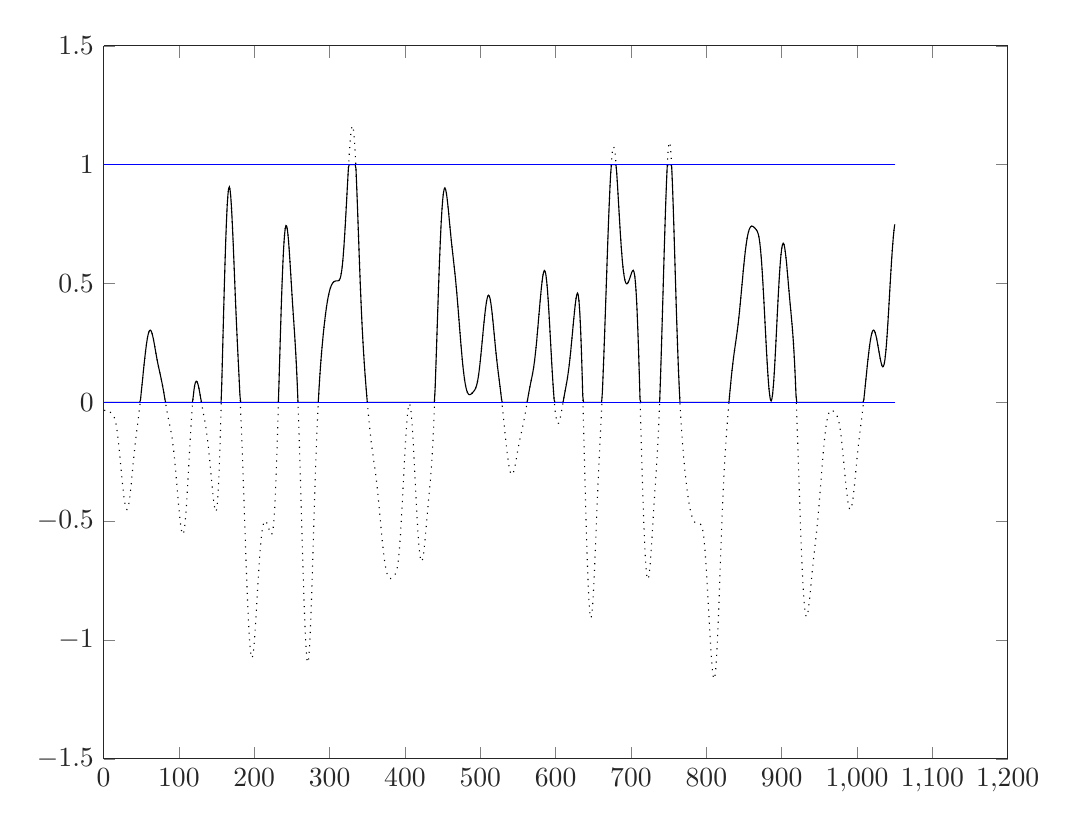
\begin{tikzpicture}

\begin{axis}[%
width=4.52083333333333in,
height=3.565625in,
scale only axis,
separate axis lines,
every outer x axis line/.append style={white!15!black},
every x tick label/.append style={font=\color{white!15!black}},
xmin=0,
xmax=1200,
every outer y axis line/.append style={white!15!black},
every y tick label/.append style={font=\color{white!15!black}},
ymin=-1.5,
ymax=1.5
]
\addplot [color=black,dotted,forget plot]
  table[row sep=crcr]{%
1	-0.0352403667366428\\
2	-0.0328038543655187\\
3	-0.0315920055619777\\
4	-0.0314897834783689\\
5	-0.0323451943730028\\
6	-0.033980940681956\\
7	-0.0362073819638487\\
8	-0.0388349765150509\\
9	-0.0416860598923207\\
10	-0.0446252757724698\\
11	-0.0476496219981174\\
12	-0.0510234881169469\\
13	-0.0553487628483466\\
14	-0.0614882919839537\\
15	-0.070383367246686\\
16	-0.0828560103845895\\
17	-0.0994554237486997\\
18	-0.120371141581364\\
19	-0.145413343661888\\
20	-0.174048472105405\\
21	-0.205473063442276\\
22	-0.238707988976374\\
23	-0.272697591459755\\
24	-0.306400477467701\\
25	-0.338843677386331\\
26	-0.369094409091013\\
27	-0.39616279677214\\
28	-0.418946890257929\\
29	-0.43630495638408\\
30	-0.447218643083903\\
31	-0.450960887490186\\
32	-0.447213671616349\\
33	-0.436117039200636\\
34	-0.418252129299945\\
35	-0.394572458628329\\
36	-0.366302125230984\\
37	-0.334819478228673\\
38	-0.301542228177483\\
39	-0.267824860618901\\
40	-0.234857660943247\\
41	-0.203533404695172\\
42	-0.174295336445239\\
43	-0.147064483455502\\
44	-0.121317264150087\\
45	-0.0962723230528574\\
46	-0.0710998089701174\\
47	-0.0450951009942012\\
48	-0.0177930146290968\\
49	0.0109807067005646\\
50	0.0411118467874923\\
51	0.0722398477578173\\
52	0.103824048312423\\
53	0.135219929978378\\
54	0.165753365575636\\
55	0.194773801583412\\
56	0.221658967983065\\
57	0.245777045609962\\
58	0.266466576009615\\
59	0.28308069439652\\
60	0.295076522669545\\
61	0.302103692814132\\
62	0.304063099994009\\
63	0.301126757680675\\
64	0.293721150018402\\
65	0.282482567177641\\
66	0.268195142640202\\
67	0.251722051202619\\
68	0.23393876386275\\
69	0.215674264505155\\
70	0.197653325282861\\
71	0.180419125299796\\
72	0.164244172105257\\
73	0.149088254251521\\
74	0.134645990699175\\
75	0.120459389840247\\
76	0.106043440050803\\
77	0.0909900463254164\\
78	0.0750360434556311\\
79	0.0580934761066291\\
80	0.0402474857581388\\
81	0.0217304523732866\\
82	0.00288172374321047\\
83	-0.0158983718954113\\
84	-0.0341945530930896\\
85	-0.0516396837636372\\
86	-0.0680370808864163\\
87	-0.0835248556651831\\
88	-0.0986622193763831\\
89	-0.11434922845973\\
90	-0.131625466571666\\
91	-0.151448046179553\\
92	-0.174515115441567\\
93	-0.201160771913382\\
94	-0.231323014915939\\
95	-0.264572677934842\\
96	-0.300185330664613\\
97	-0.337237075365474\\
98	-0.37470756700828\\
99	-0.411575104624113\\
100	-0.446860009433577\\
101	-0.479539847422296\\
102	-0.50836008941867\\
103	-0.531731495642033\\
104	-0.547858909272917\\
105	-0.555035929795813\\
106	-0.551953866797672\\
107	-0.537927447416891\\
108	-0.513002808923331\\
109	-0.477950621625503\\
110	-0.434167534067386\\
111	-0.383517261682411\\
112	-0.32814297773165\\
113	-0.270278208125391\\
114	-0.212077496742455\\
115	-0.155491259620242\\
116	-0.102214105630053\\
117	-0.0536997827741382\\
118	-0.0111795678683123\\
119	0.0243665897019767\\
120	0.0522716466253436\\
121	0.0722343602886339\\
122	0.0843388073881051\\
123	0.0890349354105907\\
124	0.0870852791163751\\
125	0.0794882322208531\\
126	0.0673897269584738\\
127	0.0519942126821553\\
128	0.0344837995056857\\
129	0.0159504759010131\\
130	-0.00267539952428472\\
131	-0.0207407370629656\\
132	-0.038015833834885\\
133	-0.0547630801894654\\
134	-0.0716491758521005\\
135	-0.0895444013093755\\
136	-0.109302489993281\\
137	-0.131582957452529\\
138	-0.156740467774279\\
139	-0.184783259638981\\
140	-0.215389812856595\\
141	-0.247967295852939\\
142	-0.2817340853326\\
143	-0.315811121844732\\
144	-0.349305662681079\\
145	-0.381305732709256\\
146	-0.410630069312462\\
147	-0.435384914708668\\
148	-0.4527289411886\\
149	-0.459147360249905\\
150	-0.451092498636041\\
151	-0.425666483013333\\
152	-0.381135664856494\\
153	-0.317199744752144\\
154	-0.235017927541791\\
155	-0.137038215939671\\
156	-0.0266939714640592\\
157	0.0919665067334283\\
158	0.214660527844968\\
159	0.337215262352073\\
160	0.455799172346766\\
161	0.566927822431712\\
162	0.667275177214401\\
163	0.753556227150809\\
164	0.822686484168853\\
165	0.872138075384665\\
166	0.900294878905336\\
167	0.906682617918634\\
168	0.892034890524372\\
169	0.858205565722197\\
170	0.807964019858041\\
171	0.744719148310923\\
172	0.672216820777533\\
173	0.594248707321437\\
174	0.514397016113813\\
175	0.435777342749641\\
176	0.360674350121192\\
177	0.290109696952432\\
178	0.223636477493611\\
179	0.159574296911303\\
180	0.095563709722127\\
181	0.029181918188819\\
182	-0.0415519913451103\\
183	-0.117852109406084\\
184	-0.200028910641833\\
185	-0.287512969395104\\
186	-0.37899545290207\\
187	-0.47263815611585\\
188	-0.566310588083926\\
189	-0.657818168992844\\
190	-0.74506460662362\\
191	-0.826066633836737\\
192	-0.89883936359757\\
193	-0.96133359652876\\
194	-1.0115652778858\\
195	-1.04788001637776\\
196	-1.06921490960691\\
197	-1.07527122966523\\
198	-1.06657077001674\\
199	-1.04440314659256\\
200	-1.01068957323817\\
201	-0.967795247379479\\
202	-0.918321763266946\\
203	-0.86490590240421\\
204	-0.81004451306179\\
205	-0.755963016733282\\
206	-0.704544162250647\\
207	-0.657312900624055\\
208	-0.615443152884008\\
209	-0.579757297862567\\
210	-0.550721276867719\\
211	-0.528451639020882\\
212	-0.512742872131165\\
213	-0.503114429627671\\
214	-0.498872270209535\\
215	-0.499177851410514\\
216	-0.503117597974134\\
217	-0.509766799506426\\
218	-0.518244131066914\\
219	-0.527750715153155\\
220	-0.537527110827421\\
221	-0.546593488846809\\
222	-0.553322282689155\\
223	-0.555205942296735\\
224	-0.549090948990938\\
225	-0.531748963478696\\
226	-0.500491941799577\\
227	-0.453640372867949\\
228	-0.390773737955442\\
229	-0.312763845520866\\
230	-0.221631308602613\\
231	-0.120281935571447\\
232	-0.0121815218067753\\
233	0.098980094730799\\
234	0.20959472748152\\
235	0.316354058029553\\
236	0.416302718194506\\
237	0.506745460346729\\
238	0.585183260790587\\
239	0.649415233794336\\
240	0.697757186110702\\
241	0.729251252548386\\
242	0.743788980797554\\
243	0.742125447344262\\
244	0.725793754324686\\
245	0.696945627101284\\
246	0.658149401201937\\
247	0.61217519513385\\
248	0.561792439648992\\
249	0.509593961546378\\
250	0.457791498145272\\
251	0.407851615544578\\
252	0.360018850508571\\
253	0.313081848646791\\
254	0.264644163181455\\
255	0.211759976651083\\
256	0.151631076192911\\
257	0.0821647195371414\\
258	0.00231353143739392\\
259	-0.0878080500586278\\
260	-0.186994747690699\\
261	-0.293154573785872\\
262	-0.403588519708789\\
263	-0.515294912738075\\
264	-0.625254501758353\\
265	-0.730604420663081\\
266	-0.828553699554227\\
267	-0.916081313052034\\
268	-0.989769827093519\\
269	-1.04604407557994\\
270	-1.08169838964205\\
271	-1.09443791563171\\
272	-1.08325913283764\\
273	-1.04861037640394\\
274	-0.992341185032547\\
275	-0.917485902479111\\
276	-0.827941095984308\\
277	-0.728096071552267\\
278	-0.622467198741267\\
279	-0.51537302889915\\
280	-0.410657977166594\\
281	-0.311442345577506\\
282	-0.219911766569581\\
283	-0.137229527261297\\
284	-0.0636271921158999\\
285	0.00137379601124384\\
286	0.0586984648859942\\
287	0.109475001475951\\
288	0.154842177115535\\
289	0.195817421643663\\
290	0.233222759074039\\
291	0.267658974660067\\
292	0.299515559864146\\
293	0.329003821786681\\
294	0.356201968934234\\
295	0.381103219016517\\
296	0.403660460166843\\
297	0.423823374038501\\
298	0.441565979593611\\
299	0.456904177879043\\
300	0.469904043409883\\
301	0.480682349000474\\
302	0.489401183100897\\
303	0.496258606611068\\
304	0.501477163029112\\
305	0.505291806706999\\
306	0.507938446187966\\
307	0.50964403182771\\
308	0.510618455713807\\
309	0.511050361320239\\
310	0.511141522581073\\
311	0.511250933910325\\
312	0.512123026001023\\
313	0.515009316645183\\
314	0.521541220633984\\
315	0.533423039401608\\
316	0.552100676201736\\
317	0.578507517548137\\
318	0.612925474227257\\
319	0.65496126685228\\
320	0.703616970957612\\
321	0.757425026882826\\
322	0.814616808194429\\
323	0.873298118639386\\
324	0.931607897487924\\
325	0.9877932275013\\
326	1.04008429747246\\
327	1.08640593765295\\
328	1.12421846348138\\
329	1.15070949282505\\
330	1.16323752832301\\
331	1.15979664416669\\
332	1.13935403180591\\
333	1.10200826555424\\
334	1.04897296873843\\
335	0.982421472246392\\
336	0.905240384043001\\
337	0.820740322153669\\
338	0.73236551558397\\
339	0.64343272843217\\
340	0.556901671236925\\
341	0.475149506900871\\
342	0.399764345903192\\
343	0.331453059627787\\
344	0.27012899233419\\
345	0.215131677805216\\
346	0.165484516586597\\
347	0.120125498377832\\
348	0.0780809479035699\\
349	0.0385742292769399\\
350	0.00107459361360342\\
351	-0.0347018376728271\\
352	-0.0688245927434401\\
353	-0.101200733153964\\
354	-0.131635218170699\\
355	-0.15991063683397\\
356	-0.185921348784184\\
357	-0.209843841909681\\
358	-0.232231813291755\\
359	-0.253954230148923\\
360	-0.276018111431399\\
361	-0.299368512929115\\
362	-0.324727102288112\\
363	-0.352493892587646\\
364	-0.382714445548739\\
365	-0.415102236545234\\
366	-0.449100262360041\\
367	-0.483964924743464\\
368	-0.518856999610238\\
369	-0.552927593320027\\
370	-0.585388968060192\\
371	-0.615561766731557\\
372	-0.642898328624319\\
373	-0.666992864216651\\
374	-0.687588367460805\\
375	-0.704579999474918\\
376	-0.718010516135817\\
377	-0.728056100992394\\
378	-0.735003917483043\\
379	-0.739224116242189\\
380	-0.741139453715928\\
381	-0.741195497987904\\
382	-0.739833728550567\\
383	-0.737469441839592\\
384	-0.734473391348352\\
385	-0.731120898222768\\
386	-0.727433047370774\\
387	-0.72293589826587\\
388	-0.71653713852378\\
389	-0.706668528510155\\
390	-0.691620095534375\\
391	-0.669901088778528\\
392	-0.640519859112557\\
393	-0.603141845947974\\
394	-0.558124999429599\\
395	-0.506454363257767\\
396	-0.449607029665501\\
397	-0.389379963931194\\
398	-0.327708976537929\\
399	-0.266503074358295\\
400	-0.20754748136994\\
401	-0.152562301427374\\
402	-0.103391211163085\\
403	-0.0621077024706759\\
404	-0.0308768875099581\\
405	-0.0116426712578227\\
406	-0.00580506359413621\\
407	-0.0139927715224783\\
408	-0.0359668497376295\\
409	-0.070650400230947\\
410	-0.116257317376274\\
411	-0.170484588019177\\
412	-0.230732698219853\\
413	-0.29432408308406\\
414	-0.358695798369115\\
415	-0.421530038260706\\
416	-0.480770513135201\\
417	-0.534539967708987\\
418	-0.581083019699239\\
419	-0.61883096017179\\
420	-0.646553311226952\\
421	-0.66350669964973\\
422	-0.669525293830655\\
423	-0.665036014993706\\
424	-0.651004245513922\\
425	-0.628827452757942\\
426	-0.600198260574518\\
427	-0.566957599337326\\
428	-0.530955560209164\\
429	-0.493929350511918\\
430	-0.457349278225369\\
431	-0.422119413728099\\
432	-0.38817358099587\\
433	-0.354273981849216\\
434	-0.318239085298073\\
435	-0.2774819184853\\
436	-0.229598717768079\\
437	-0.172836722833976\\
438	-0.106374306387258\\
439	-0.0304095736640676\\
440	0.0539109631173334\\
441	0.144676538508324\\
442	0.239459453621495\\
443	0.335581516312056\\
444	0.43036381265302\\
445	0.521315887927478\\
446	0.606209613962229\\
447	0.683047880271862\\
448	0.75004071289309\\
449	0.805678166639476\\
450	0.848869807811485\\
451	0.87907163094692\\
452	0.89635239146346\\
453	0.90138694785565\\
454	0.895384479307032\\
455	0.879969672918048\\
456	0.85703815652661\\
457	0.828606143962353\\
458	0.796670743571619\\
459	0.763091146447972\\
460	0.729473610653506\\
461	0.697013758811368\\
462	0.666312357349394\\
463	0.637291207171048\\
464	0.609301134807352\\
465	0.581368856053643\\
466	0.552470329163217\\
467	0.521755788343499\\
468	0.488695930668701\\
469	0.453145709398077\\
470	0.415337656017927\\
471	0.375823713173862\\
472	0.335386101166612\\
473	0.294935832973381\\
474	0.255413910656997\\
475	0.217707595483278\\
476	0.182591801427695\\
477	0.150696858403962\\
478	0.122492274457376\\
479	0.0982765997249449\\
480	0.0781733499514658\\
481	0.0621369339105014\\
482	0.0499696639807892\\
483	0.0413479732105406\\
484	0.0358545953321696\\
485	0.0330131221468414\\
486	0.0323216493070103\\
487	0.0332829520935878\\
488	0.0354292761253555\\
489	0.0383418860019277\\
490	0.041685234999105\\
491	0.0452974217913434\\
492	0.0493230782578662\\
493	0.0542795264572149\\
494	0.0609751832570959\\
495	0.0703214942118476\\
496	0.0831296461747006\\
497	0.0999517937925001\\
498	0.120989581632888\\
499	0.146070566968916\\
500	0.174680739947207\\
501	0.206036040484635\\
502	0.239175002241243\\
503	0.27305691670737\\
504	0.306652164690864\\
505	0.338996310372155\\
506	0.369162082097369\\
507	0.396162490897778\\
508	0.418896347067514\\
509	0.436221078598118\\
510	0.447116401738103\\
511	0.45085268071249\\
512	0.447109060023701\\
513	0.436022774376649\\
514	0.41817239221981\\
515	0.394509231670893\\
516	0.366255632232249\\
517	0.33478863990958\\
518	0.301525093646824\\
519	0.267818988340622\\
520	0.234860433778247\\
521	0.203542272926162\\
522	0.174307989889094\\
523	0.147078958892002\\
524	0.121331997530129\\
525	0.0962861575685196\\
526	0.071111970395942\\
527	0.045105151075549\\
528	0.017800792012746\\
529	-0.010975150150185\\
530	-0.0411083082378435\\
531	-0.0722380299368309\\
532	-0.103823607633319\\
533	-0.135220514945489\\
534	-0.165754645248331\\
535	-0.194775484685027\\
536	-0.22166081378529\\
537	-0.245778868032282\\
538	-0.266468242489192\\
539	-0.283082121050593\\
540	-0.295077667133479\\
541	-0.302104545933222\\
542	-0.304063677309575\\
543	-0.301127091407825\\
544	-0.29372128198396\\
545	-0.282482542985448\\
546	-0.268195007164954\\
547	-0.251721845385415\\
548	-0.233938522690768\\
549	-0.215674016001002\\
550	-0.197653090301059\\
551	-0.180418917922818\\
552	-0.16424400044353\\
553	-0.149088121475263\\
554	-0.134645896159928\\
555	-0.120459330172404\\
556	-0.106043410175231\\
557	-0.0909900403061776\\
558	-0.0750360551854428\\
559	-0.0580934998163822\\
560	-0.0402475163604118\\
561	-0.0217304856596043\\
562	-0.0028817564604336\\
563	0.0158983420620371\\
564	0.0341945276032243\\
565	0.0516396633468902\\
566	0.0680370656881779\\
567	0.0835248453964836\\
568	0.098662213455333\\
569	0.11434922613616\\
570	0.131625467030166\\
571	0.151448048619069\\
572	0.174515119131988\\
573	0.201160776231187\\
574	0.231323019361959\\
575	0.264572682137739\\
576	0.300185334373728\\
577	0.337237078436532\\
578	0.374707569384987\\
579	0.411575106318169\\
580	0.446860010505062\\
581	0.479539847961796\\
582	0.508360089532027\\
583	0.531731495438138\\
584	0.547858908854637\\
585	0.555035929253878\\
586	0.551953866207156\\
587	0.537927446835855\\
588	0.513002808393117\\
589	0.477950621172216\\
590	0.434167533704122\\
591	0.38351726141185\\
592	0.328142977548723\\
593	0.2702782080198\\
594	0.212077496700892\\
595	0.155491259628224\\
596	0.102214105673343\\
597	0.05369978283975\\
598	0.0111795679451527\\
599	-0.0243665896227944\\
600	-0.0522716465504352\\
601	-0.0722343602224685\\
602	-0.0843388073332613\\
603	-0.0890349353680802\\
604	-0.087085279086001\\
605	-0.0794882322015556\\
606	-0.0673897269486493\\
607	-0.0519942126799281\\
608	-0.0344837995091243\\
609	-0.0159504759082928\\
610	0.00267539951477454\\
611	0.0207407370525577\\
612	0.0380158338246098\\
613	0.0547630801800578\\
614	0.0716491758440241\\
615	0.0895444013028642\\
616	0.109302489988382\\
617	0.131582957449155\\
618	0.156740467772249\\
619	0.18478325963806\\
620	0.215389812856529\\
621	0.247967295853479\\
622	0.281734085333518\\
623	0.315811121845835\\
624	0.349305662682213\\
625	0.381305732710308\\
626	0.410630069313356\\
627	0.435384914709363\\
628	0.452728941189082\\
629	0.459147360250181\\
630	0.451092498636132\\
631	0.42566648301327\\
632	0.381135664856312\\
633	0.317199744751881\\
634	0.235017927541478\\
635	0.137038215939339\\
636	0.0266939714637309\\
637	-0.0919665067337347\\
638	-0.214660527845239\\
639	-0.337215262352303\\
640	-0.455799172346949\\
641	-0.56692782243185\\
642	-0.667275177214496\\
643	-0.753556227150864\\
644	-0.822686484168875\\
645	-0.872138075384659\\
646	-0.900294878905307\\
647	-0.906682617918585\\
648	-0.89203489052431\\
649	-0.858205565722124\\
650	-0.80796401985796\\
651	-0.744719148310836\\
652	-0.672216820777443\\
653	-0.594248707321344\\
654	-0.514397016113718\\
655	-0.435777342749546\\
656	-0.360674350121098\\
657	-0.29010969695234\\
658	-0.223636477493521\\
659	-0.159574296911215\\
660	-0.0955637097220432\\
661	-0.029181918188739\\
662	0.0415519913451864\\
663	0.117852109406156\\
664	0.2000289106419\\
665	0.287512969395168\\
666	0.37899545290213\\
667	0.472638156115908\\
668	0.566310588083982\\
669	0.657818168992899\\
670	0.745064606623675\\
671	0.826066633836793\\
672	0.898839363597627\\
673	0.961333596528819\\
674	1.01156527788586\\
675	1.04788001637782\\
676	1.06921490960697\\
677	1.0752712296653\\
678	1.0665707700168\\
679	1.04440314659262\\
680	1.01068957323823\\
681	0.96779524737954\\
682	0.918321763267003\\
683	0.864905902404259\\
684	0.810044513061832\\
685	0.755963016733315\\
686	0.70454416225067\\
687	0.657312900624066\\
688	0.615443152884008\\
689	0.579757297862554\\
690	0.550721276867693\\
691	0.528451639020843\\
692	0.512742872131114\\
693	0.503114429627608\\
694	0.498872270209461\\
695	0.499177851410428\\
696	0.503117597974039\\
697	0.509766799506322\\
698	0.518244131066802\\
699	0.527750715153036\\
700	0.537527110827296\\
701	0.546593488846679\\
702	0.55332228268902\\
703	0.555205942296595\\
704	0.549090948990795\\
705	0.53174896347855\\
706	0.500491941799428\\
707	0.453640372867797\\
708	0.390773737955288\\
709	0.312763845520711\\
710	0.221631308602459\\
711	0.120281935571292\\
712	0.0121815218066224\\
713	-0.0989800947309485\\
714	-0.209594727481666\\
715	-0.316354058029692\\
716	-0.416302718194638\\
717	-0.506745460346852\\
718	-0.5851832607907\\
719	-0.649415233794438\\
720	-0.697757186110793\\
721	-0.729251252548465\\
722	-0.743788980797623\\
723	-0.742125447344321\\
724	-0.725793754324737\\
725	-0.696945627101327\\
726	-0.658149401201976\\
727	-0.612175195133886\\
728	-0.561792439649027\\
729	-0.509593961546415\\
730	-0.457791498145313\\
731	-0.407851615544623\\
732	-0.360018850508622\\
733	-0.313081848646848\\
734	-0.264644163181519\\
735	-0.211759976651153\\
736	-0.151631076192987\\
737	-0.082164719537222\\
738	-0.00231353143747802\\
739	0.0878080500585416\\
740	0.186994747690612\\
741	0.293154573785785\\
742	0.403588519708704\\
743	0.515294912737992\\
744	0.625254501758271\\
745	0.730604420663002\\
746	0.828553699554149\\
747	0.916081313051956\\
748	0.98976982709344\\
749	1.04604407557986\\
750	1.08169838964196\\
751	1.09443791563162\\
752	1.08325913283754\\
753	1.04861037640384\\
754	0.992341185032437\\
755	0.917485902478994\\
756	0.827941095984183\\
757	0.728096071552135\\
758	0.622467198741129\\
759	0.515373028899008\\
760	0.410657977166449\\
761	0.311442345577359\\
762	0.219911766569434\\
763	0.137229527261153\\
764	0.0636271921157609\\
765	-0.00137379601137605\\
766	-0.0586984648861178\\
767	-0.109475001476064\\
768	-0.154842177115636\\
769	-0.195817421643752\\
770	-0.233222759074113\\
771	-0.267658974660127\\
772	-0.299515559864191\\
773	-0.329003821786711\\
774	-0.356201968934249\\
775	-0.381103219016517\\
776	-0.403660460166828\\
777	-0.423823374038473\\
778	-0.441565979593569\\
779	-0.45690417787899\\
780	-0.469904043409818\\
781	-0.480682349000399\\
782	-0.489401183100814\\
783	-0.496258606610977\\
784	-0.501477163029016\\
785	-0.5052918067069\\
786	-0.507938446187864\\
787	-0.509644031827608\\
788	-0.510618455713707\\
789	-0.511050361320142\\
790	-0.511141522580981\\
791	-0.511250933910241\\
792	-0.512123026000949\\
793	-0.515009316645121\\
794	-0.521541220633936\\
795	-0.533423039401576\\
796	-0.552100676201722\\
797	-0.578507517548142\\
798	-0.612925474227284\\
799	-0.654961266852328\\
800	-0.703616970957684\\
801	-0.75742502688292\\
802	-0.814616808194546\\
803	-0.873298118639526\\
804	-0.931607897488085\\
805	-0.987793227501481\\
806	-1.04008429747266\\
807	-1.08640593765316\\
808	-1.1242184634816\\
809	-1.15070949282529\\
810	-1.16323752832326\\
811	-1.15979664416694\\
812	-1.13935403180617\\
813	-1.10200826555449\\
814	-1.04897296873868\\
815	-0.982421472246636\\
816	-0.905240384043237\\
817	-0.820740322153896\\
818	-0.732365515584186\\
819	-0.643432728432374\\
820	-0.556901671237117\\
821	-0.475149506901051\\
822	-0.399764345903361\\
823	-0.331453059627946\\
824	-0.27012899233434\\
825	-0.215131677805357\\
826	-0.165484516586732\\
827	-0.120125498377963\\
828	-0.0780809479036967\\
829	-0.0385742292770643\\
830	-0.00107459361372698\\
831	0.0347018376727047\\
832	0.0688245927433174\\
833	0.101200733153842\\
834	0.131635218170577\\
835	0.15991063683385\\
836	0.185921348784066\\
837	0.209843841909568\\
838	0.232231813291648\\
839	0.253954230148822\\
840	0.276018111431307\\
841	0.299368512929033\\
842	0.324727102288041\\
843	0.352493892587586\\
844	0.382714445548691\\
845	0.415102236545198\\
846	0.449100262360017\\
847	0.48396492474345\\
848	0.518856999610233\\
849	0.552927593320031\\
850	0.585388968060203\\
851	0.615561766731574\\
852	0.642898328624342\\
853	0.666992864216678\\
854	0.687588367460836\\
855	0.704579999474953\\
856	0.718010516135856\\
857	0.728056100992439\\
858	0.735003917483093\\
859	0.739224116242246\\
860	0.741139453715992\\
861	0.741195497987977\\
862	0.739833728550647\\
863	0.737469441839679\\
864	0.734473391348446\\
865	0.731120898222868\\
866	0.727433047370878\\
867	0.722935898265974\\
868	0.716537138523883\\
869	0.706668528510253\\
870	0.691620095534464\\
871	0.669901088778605\\
872	0.640519859112621\\
873	0.603141845948021\\
874	0.558124999429627\\
875	0.506454363257774\\
876	0.449607029665486\\
877	0.389379963931158\\
878	0.327708976537872\\
879	0.266503074358218\\
880	0.207547481369846\\
881	0.152562301427265\\
882	0.103391211162962\\
883	0.0621077024705431\\
884	0.0308768875098172\\
885	0.0116426712576768\\
886	0.00580506359398707\\
887	0.0139927715223282\\
888	0.0359668497374802\\
889	0.0706504002307993\\
890	0.11625731737613\\
891	0.170484588019038\\
892	0.230732698219718\\
893	0.294324083083932\\
894	0.358695798368995\\
895	0.421530038260594\\
896	0.4807705131351\\
897	0.534539967708897\\
898	0.581083019699163\\
899	0.618830960171729\\
900	0.646553311226908\\
901	0.663506699649704\\
902	0.669525293830649\\
903	0.665036014993722\\
904	0.651004245513959\\
905	0.628827452758\\
906	0.600198260574596\\
907	0.566957599337423\\
908	0.530955560209277\\
909	0.493929350512045\\
910	0.457349278225505\\
911	0.422119413728242\\
912	0.388173580996015\\
913	0.354273981849358\\
914	0.31823908529821\\
915	0.277481918485426\\
916	0.229598717768191\\
917	0.172836722834071\\
918	0.106374306387333\\
919	0.0304095736641224\\
920	-0.0539109631172999\\
921	-0.144676538508312\\
922	-0.239459453621502\\
923	-0.335581516312081\\
924	-0.430363812653059\\
925	-0.52131588792753\\
926	-0.606209613962291\\
927	-0.68304788027193\\
928	-0.750040712893161\\
929	-0.805678166639547\\
930	-0.848869807811552\\
931	-0.879071630946982\\
932	-0.896352391463516\\
933	-0.901386947855698\\
934	-0.895384479307073\\
935	-0.87996967291808\\
936	-0.857038156526634\\
937	-0.828606143962369\\
938	-0.796670743571628\\
939	-0.763091146447976\\
940	-0.729473610653505\\
941	-0.697013758811363\\
942	-0.666312357349387\\
943	-0.637291207171038\\
944	-0.609301134807341\\
945	-0.58136885605363\\
946	-0.552470329163202\\
947	-0.521755788343482\\
948	-0.488695930668683\\
949	-0.453145709398057\\
950	-0.415337656017904\\
951	-0.375823713173836\\
952	-0.335386101166584\\
953	-0.29493583297335\\
954	-0.255413910656964\\
955	-0.217707595483243\\
956	-0.182591801427658\\
957	-0.150696858403925\\
958	-0.122492274457339\\
959	-0.0982765997249075\\
960	-0.0781733499514297\\
961	-0.0621369339104666\\
962	-0.0499696639807561\\
963	-0.0413479732105085\\
964	-0.0358545953321395\\
965	-0.0330131221468128\\
966	-0.0323216493069837\\
967	-0.0332829520935626\\
968	-0.035429276125332\\
969	-0.0383418860019053\\
970	-0.0416852349990852\\
971	-0.0452974217913252\\
972	-0.0493230782578519\\
973	-0.0542795264572039\\
974	-0.0609751832570911\\
975	-0.0703214942118483\\
976	-0.0831296461747114\\
977	-0.0999517937925194\\
978	-0.120989581632921\\
979	-0.146070566968961\\
980	-0.174680739947269\\
981	-0.206036040484712\\
982	-0.23917500224134\\
983	-0.273056916707483\\
984	-0.306652164691\\
985	-0.338996310372305\\
986	-0.369162082097542\\
987	-0.396162490897963\\
988	-0.41889634706772\\
989	-0.436221078598331\\
990	-0.447116401738335\\
991	-0.450852680712722\\
992	-0.44710906002395\\
993	-0.436022774376888\\
994	-0.418172392220066\\
995	-0.394509231671127\\
996	-0.366255632232502\\
997	-0.334788639909797\\
998	-0.301525093647064\\
999	-0.267818988340807\\
1000	-0.234860433778467\\
1001	-0.203542272926303\\
1002	-0.17430798988929\\
1003	-0.147078958892082\\
1004	-0.121331997530306\\
1005	-0.0962861575685227\\
1006	-0.0711119703961128\\
1007	-0.0451051510754476\\
1008	-0.0178007920129444\\
1009	0.0109751501504374\\
1010	0.0411083082375464\\
1011	0.0722380299373302\\
1012	0.103823607632769\\
1013	0.135220514946454\\
1014	0.165754645247167\\
1015	0.194775484687005\\
1016	0.221660813782587\\
1017	0.245778868036812\\
1018	0.26646824248222\\
1019	0.283082121062631\\
1020	0.295077667112676\\
1021	0.302104545972175\\
1022	0.304063677232649\\
1023	0.301127091573691\\
1024	0.29372128158877\\
1025	0.282482544061506\\
1026	0.268195003665684\\
1027	0.251721860037789\\
1028	0.233938431500787\\
1029	0.21567526348113\\
1030	0.197708196619704\\
1031	0.180864784116396\\
1032	0.166223090235151\\
1033	0.155221194761011\\
1034	0.149540744271029\\
1035	0.150827615189522\\
1036	0.160394607108879\\
1037	0.178999957977964\\
1038	0.206735672305094\\
1039	0.243024134161719\\
1040	0.286701968931336\\
1041	0.336162161571369\\
1042	0.389524868223126\\
1043	0.444811362675721\\
1044	0.500100961744264\\
1045	0.553647102003322\\
1046	0.603923431307901\\
1047	0.649606546340879\\
1048	0.689558105829513\\
1049	0.722856415525642\\
1050	0.748862315446572\\
};
\addplot [color=black,solid,forget plot]
  table[row sep=crcr]{%
1	0\\
2	0\\
3	0\\
4	0\\
5	0\\
6	0\\
7	0\\
8	0\\
9	0\\
10	0\\
11	0\\
12	0\\
13	0\\
14	0\\
15	0\\
16	0\\
17	0\\
18	0\\
19	0\\
20	0\\
21	0\\
22	0\\
23	0\\
24	0\\
25	0\\
26	0\\
27	0\\
28	0\\
29	0\\
30	0\\
31	0\\
32	0\\
33	0\\
34	0\\
35	0\\
36	0\\
37	0\\
38	0\\
39	0\\
40	0\\
41	0\\
42	0\\
43	0\\
44	0\\
45	0\\
46	0\\
47	0\\
48	0\\
49	0.0109807067005646\\
50	0.0411118467874923\\
51	0.0722398477578173\\
52	0.103824048312423\\
53	0.135219929978378\\
54	0.165753365575636\\
55	0.194773801583412\\
56	0.221658967983065\\
57	0.245777045609962\\
58	0.266466576009615\\
59	0.28308069439652\\
60	0.295076522669545\\
61	0.302103692814132\\
62	0.304063099994009\\
63	0.301126757680675\\
64	0.293721150018402\\
65	0.282482567177641\\
66	0.268195142640202\\
67	0.251722051202619\\
68	0.23393876386275\\
69	0.215674264505155\\
70	0.197653325282861\\
71	0.180419125299796\\
72	0.164244172105257\\
73	0.149088254251521\\
74	0.134645990699175\\
75	0.120459389840247\\
76	0.106043440050803\\
77	0.0909900463254164\\
78	0.0750360434556311\\
79	0.0580934761066291\\
80	0.0402474857581388\\
81	0.0217304523732866\\
82	0.00288172374321047\\
83	0\\
84	0\\
85	0\\
86	0\\
87	0\\
88	0\\
89	0\\
90	0\\
91	0\\
92	0\\
93	0\\
94	0\\
95	0\\
96	0\\
97	0\\
98	0\\
99	0\\
100	0\\
101	0\\
102	0\\
103	0\\
104	0\\
105	0\\
106	0\\
107	0\\
108	0\\
109	0\\
110	0\\
111	0\\
112	0\\
113	0\\
114	0\\
115	0\\
116	0\\
117	0\\
118	0\\
119	0.0243665897019767\\
120	0.0522716466253436\\
121	0.0722343602886339\\
122	0.0843388073881051\\
123	0.0890349354105907\\
124	0.0870852791163751\\
125	0.0794882322208531\\
126	0.0673897269584738\\
127	0.0519942126821553\\
128	0.0344837995056857\\
129	0.0159504759010131\\
130	0\\
131	0\\
132	0\\
133	0\\
134	0\\
135	0\\
136	0\\
137	0\\
138	0\\
139	0\\
140	0\\
141	0\\
142	0\\
143	0\\
144	0\\
145	0\\
146	0\\
147	0\\
148	0\\
149	0\\
150	0\\
151	0\\
152	0\\
153	0\\
154	0\\
155	0\\
156	0\\
157	0.0919665067334283\\
158	0.214660527844968\\
159	0.337215262352073\\
160	0.455799172346766\\
161	0.566927822431712\\
162	0.667275177214401\\
163	0.753556227150809\\
164	0.822686484168853\\
165	0.872138075384665\\
166	0.900294878905336\\
167	0.906682617918634\\
168	0.892034890524372\\
169	0.858205565722197\\
170	0.807964019858041\\
171	0.744719148310923\\
172	0.672216820777533\\
173	0.594248707321437\\
174	0.514397016113813\\
175	0.435777342749641\\
176	0.360674350121192\\
177	0.290109696952432\\
178	0.223636477493611\\
179	0.159574296911303\\
180	0.095563709722127\\
181	0.029181918188819\\
182	0\\
183	0\\
184	0\\
185	0\\
186	0\\
187	0\\
188	0\\
189	0\\
190	0\\
191	0\\
192	0\\
193	0\\
194	0\\
195	0\\
196	0\\
197	0\\
198	0\\
199	0\\
200	0\\
201	0\\
202	0\\
203	0\\
204	0\\
205	0\\
206	0\\
207	0\\
208	0\\
209	0\\
210	0\\
211	0\\
212	0\\
213	0\\
214	0\\
215	0\\
216	0\\
217	0\\
218	0\\
219	0\\
220	0\\
221	0\\
222	0\\
223	0\\
224	0\\
225	0\\
226	0\\
227	0\\
228	0\\
229	0\\
230	0\\
231	0\\
232	0\\
233	0.098980094730799\\
234	0.20959472748152\\
235	0.316354058029553\\
236	0.416302718194506\\
237	0.506745460346729\\
238	0.585183260790587\\
239	0.649415233794336\\
240	0.697757186110702\\
241	0.729251252548386\\
242	0.743788980797554\\
243	0.742125447344262\\
244	0.725793754324686\\
245	0.696945627101284\\
246	0.658149401201937\\
247	0.61217519513385\\
248	0.561792439648992\\
249	0.509593961546378\\
250	0.457791498145272\\
251	0.407851615544578\\
252	0.360018850508571\\
253	0.313081848646791\\
254	0.264644163181455\\
255	0.211759976651083\\
256	0.151631076192911\\
257	0.0821647195371414\\
258	0.00231353143739392\\
259	0\\
260	0\\
261	0\\
262	0\\
263	0\\
264	0\\
265	0\\
266	0\\
267	0\\
268	0\\
269	0\\
270	0\\
271	0\\
272	0\\
273	0\\
274	0\\
275	0\\
276	0\\
277	0\\
278	0\\
279	0\\
280	0\\
281	0\\
282	0\\
283	0\\
284	0\\
285	0.00137379601124384\\
286	0.0586984648859942\\
287	0.109475001475951\\
288	0.154842177115535\\
289	0.195817421643663\\
290	0.233222759074039\\
291	0.267658974660067\\
292	0.299515559864146\\
293	0.329003821786681\\
294	0.356201968934234\\
295	0.381103219016517\\
296	0.403660460166843\\
297	0.423823374038501\\
298	0.441565979593611\\
299	0.456904177879043\\
300	0.469904043409883\\
301	0.480682349000474\\
302	0.489401183100897\\
303	0.496258606611068\\
304	0.501477163029112\\
305	0.505291806706999\\
306	0.507938446187966\\
307	0.50964403182771\\
308	0.510618455713807\\
309	0.511050361320239\\
310	0.511141522581073\\
311	0.511250933910325\\
312	0.512123026001023\\
313	0.515009316645183\\
314	0.521541220633984\\
315	0.533423039401608\\
316	0.552100676201736\\
317	0.578507517548137\\
318	0.612925474227257\\
319	0.65496126685228\\
320	0.703616970957612\\
321	0.757425026882826\\
322	0.814616808194429\\
323	0.873298118639386\\
324	0.931607897487924\\
325	0.9877932275013\\
326	1\\
327	1\\
328	1\\
329	1\\
330	1\\
331	1\\
332	1\\
333	1\\
334	1\\
335	0.982421472246392\\
336	0.905240384043001\\
337	0.820740322153669\\
338	0.73236551558397\\
339	0.64343272843217\\
340	0.556901671236925\\
341	0.475149506900871\\
342	0.399764345903192\\
343	0.331453059627787\\
344	0.27012899233419\\
345	0.215131677805216\\
346	0.165484516586597\\
347	0.120125498377832\\
348	0.0780809479035699\\
349	0.0385742292769399\\
350	0.00107459361360342\\
351	0\\
352	0\\
353	0\\
354	0\\
355	0\\
356	0\\
357	0\\
358	0\\
359	0\\
360	0\\
361	0\\
362	0\\
363	0\\
364	0\\
365	0\\
366	0\\
367	0\\
368	0\\
369	0\\
370	0\\
371	0\\
372	0\\
373	0\\
374	0\\
375	0\\
376	0\\
377	0\\
378	0\\
379	0\\
380	0\\
381	0\\
382	0\\
383	0\\
384	0\\
385	0\\
386	0\\
387	0\\
388	0\\
389	0\\
390	0\\
391	0\\
392	0\\
393	0\\
394	0\\
395	0\\
396	0\\
397	0\\
398	0\\
399	0\\
400	0\\
401	0\\
402	0\\
403	0\\
404	0\\
405	0\\
406	0\\
407	0\\
408	0\\
409	0\\
410	0\\
411	0\\
412	0\\
413	0\\
414	0\\
415	0\\
416	0\\
417	0\\
418	0\\
419	0\\
420	0\\
421	0\\
422	0\\
423	0\\
424	0\\
425	0\\
426	0\\
427	0\\
428	0\\
429	0\\
430	0\\
431	0\\
432	0\\
433	0\\
434	0\\
435	0\\
436	0\\
437	0\\
438	0\\
439	0\\
440	0.0539109631173334\\
441	0.144676538508324\\
442	0.239459453621495\\
443	0.335581516312056\\
444	0.43036381265302\\
445	0.521315887927478\\
446	0.606209613962229\\
447	0.683047880271862\\
448	0.75004071289309\\
449	0.805678166639476\\
450	0.848869807811485\\
451	0.87907163094692\\
452	0.89635239146346\\
453	0.90138694785565\\
454	0.895384479307032\\
455	0.879969672918048\\
456	0.85703815652661\\
457	0.828606143962353\\
458	0.796670743571619\\
459	0.763091146447972\\
460	0.729473610653506\\
461	0.697013758811368\\
462	0.666312357349394\\
463	0.637291207171048\\
464	0.609301134807352\\
465	0.581368856053643\\
466	0.552470329163217\\
467	0.521755788343499\\
468	0.488695930668701\\
469	0.453145709398077\\
470	0.415337656017927\\
471	0.375823713173862\\
472	0.335386101166612\\
473	0.294935832973381\\
474	0.255413910656997\\
475	0.217707595483278\\
476	0.182591801427695\\
477	0.150696858403962\\
478	0.122492274457376\\
479	0.0982765997249449\\
480	0.0781733499514658\\
481	0.0621369339105014\\
482	0.0499696639807892\\
483	0.0413479732105406\\
484	0.0358545953321696\\
485	0.0330131221468414\\
486	0.0323216493070103\\
487	0.0332829520935878\\
488	0.0354292761253555\\
489	0.0383418860019277\\
490	0.041685234999105\\
491	0.0452974217913434\\
492	0.0493230782578662\\
493	0.0542795264572149\\
494	0.0609751832570959\\
495	0.0703214942118476\\
496	0.0831296461747006\\
497	0.0999517937925001\\
498	0.120989581632888\\
499	0.146070566968916\\
500	0.174680739947207\\
501	0.206036040484635\\
502	0.239175002241243\\
503	0.27305691670737\\
504	0.306652164690864\\
505	0.338996310372155\\
506	0.369162082097369\\
507	0.396162490897778\\
508	0.418896347067514\\
509	0.436221078598118\\
510	0.447116401738103\\
511	0.45085268071249\\
512	0.447109060023701\\
513	0.436022774376649\\
514	0.41817239221981\\
515	0.394509231670893\\
516	0.366255632232249\\
517	0.33478863990958\\
518	0.301525093646824\\
519	0.267818988340622\\
520	0.234860433778247\\
521	0.203542272926162\\
522	0.174307989889094\\
523	0.147078958892002\\
524	0.121331997530129\\
525	0.0962861575685196\\
526	0.071111970395942\\
527	0.045105151075549\\
528	0.017800792012746\\
529	0\\
530	0\\
531	0\\
532	0\\
533	0\\
534	0\\
535	0\\
536	0\\
537	0\\
538	0\\
539	0\\
540	0\\
541	0\\
542	0\\
543	0\\
544	0\\
545	0\\
546	0\\
547	0\\
548	0\\
549	0\\
550	0\\
551	0\\
552	0\\
553	0\\
554	0\\
555	0\\
556	0\\
557	0\\
558	0\\
559	0\\
560	0\\
561	0\\
562	0\\
563	0.0158983420620371\\
564	0.0341945276032243\\
565	0.0516396633468902\\
566	0.0680370656881779\\
567	0.0835248453964836\\
568	0.098662213455333\\
569	0.11434922613616\\
570	0.131625467030166\\
571	0.151448048619069\\
572	0.174515119131988\\
573	0.201160776231187\\
574	0.231323019361959\\
575	0.264572682137739\\
576	0.300185334373728\\
577	0.337237078436532\\
578	0.374707569384987\\
579	0.411575106318169\\
580	0.446860010505062\\
581	0.479539847961796\\
582	0.508360089532027\\
583	0.531731495438138\\
584	0.547858908854637\\
585	0.555035929253878\\
586	0.551953866207156\\
587	0.537927446835855\\
588	0.513002808393117\\
589	0.477950621172216\\
590	0.434167533704122\\
591	0.38351726141185\\
592	0.328142977548723\\
593	0.2702782080198\\
594	0.212077496700892\\
595	0.155491259628224\\
596	0.102214105673343\\
597	0.05369978283975\\
598	0.0111795679451527\\
599	0\\
600	0\\
601	0\\
602	0\\
603	0\\
604	0\\
605	0\\
606	0\\
607	0\\
608	0\\
609	0\\
610	0.00267539951477454\\
611	0.0207407370525577\\
612	0.0380158338246098\\
613	0.0547630801800578\\
614	0.0716491758440241\\
615	0.0895444013028642\\
616	0.109302489988382\\
617	0.131582957449155\\
618	0.156740467772249\\
619	0.18478325963806\\
620	0.215389812856529\\
621	0.247967295853479\\
622	0.281734085333518\\
623	0.315811121845835\\
624	0.349305662682213\\
625	0.381305732710308\\
626	0.410630069313356\\
627	0.435384914709363\\
628	0.452728941189082\\
629	0.459147360250181\\
630	0.451092498636132\\
631	0.42566648301327\\
632	0.381135664856312\\
633	0.317199744751881\\
634	0.235017927541478\\
635	0.137038215939339\\
636	0.0266939714637309\\
637	0\\
638	0\\
639	0\\
640	0\\
641	0\\
642	0\\
643	0\\
644	0\\
645	0\\
646	0\\
647	0\\
648	0\\
649	0\\
650	0\\
651	0\\
652	0\\
653	0\\
654	0\\
655	0\\
656	0\\
657	0\\
658	0\\
659	0\\
660	0\\
661	0\\
662	0.0415519913451864\\
663	0.117852109406156\\
664	0.2000289106419\\
665	0.287512969395168\\
666	0.37899545290213\\
667	0.472638156115908\\
668	0.566310588083982\\
669	0.657818168992899\\
670	0.745064606623675\\
671	0.826066633836793\\
672	0.898839363597627\\
673	0.961333596528819\\
674	1\\
675	1\\
676	1\\
677	1\\
678	1\\
679	1\\
680	1\\
681	0.96779524737954\\
682	0.918321763267003\\
683	0.864905902404259\\
684	0.810044513061832\\
685	0.755963016733315\\
686	0.70454416225067\\
687	0.657312900624066\\
688	0.615443152884008\\
689	0.579757297862554\\
690	0.550721276867693\\
691	0.528451639020843\\
692	0.512742872131114\\
693	0.503114429627608\\
694	0.498872270209461\\
695	0.499177851410428\\
696	0.503117597974039\\
697	0.509766799506322\\
698	0.518244131066802\\
699	0.527750715153036\\
700	0.537527110827296\\
701	0.546593488846679\\
702	0.55332228268902\\
703	0.555205942296595\\
704	0.549090948990795\\
705	0.53174896347855\\
706	0.500491941799428\\
707	0.453640372867797\\
708	0.390773737955288\\
709	0.312763845520711\\
710	0.221631308602459\\
711	0.120281935571292\\
712	0.0121815218066224\\
713	0\\
714	0\\
715	0\\
716	0\\
717	0\\
718	0\\
719	0\\
720	0\\
721	0\\
722	0\\
723	0\\
724	0\\
725	0\\
726	0\\
727	0\\
728	0\\
729	0\\
730	0\\
731	0\\
732	0\\
733	0\\
734	0\\
735	0\\
736	0\\
737	0\\
738	0\\
739	0.0878080500585416\\
740	0.186994747690612\\
741	0.293154573785785\\
742	0.403588519708704\\
743	0.515294912737992\\
744	0.625254501758271\\
745	0.730604420663002\\
746	0.828553699554149\\
747	0.916081313051956\\
748	0.98976982709344\\
749	1\\
750	1\\
751	1\\
752	1\\
753	1\\
754	0.992341185032437\\
755	0.917485902478994\\
756	0.827941095984183\\
757	0.728096071552135\\
758	0.622467198741129\\
759	0.515373028899008\\
760	0.410657977166449\\
761	0.311442345577359\\
762	0.219911766569434\\
763	0.137229527261153\\
764	0.0636271921157609\\
765	0\\
766	0\\
767	0\\
768	0\\
769	0\\
770	0\\
771	0\\
772	0\\
773	0\\
774	0\\
775	0\\
776	0\\
777	0\\
778	0\\
779	0\\
780	0\\
781	0\\
782	0\\
783	0\\
784	0\\
785	0\\
786	0\\
787	0\\
788	0\\
789	0\\
790	0\\
791	0\\
792	0\\
793	0\\
794	0\\
795	0\\
796	0\\
797	0\\
798	0\\
799	0\\
800	0\\
801	0\\
802	0\\
803	0\\
804	0\\
805	0\\
806	0\\
807	0\\
808	0\\
809	0\\
810	0\\
811	0\\
812	0\\
813	0\\
814	0\\
815	0\\
816	0\\
817	0\\
818	0\\
819	0\\
820	0\\
821	0\\
822	0\\
823	0\\
824	0\\
825	0\\
826	0\\
827	0\\
828	0\\
829	0\\
830	0\\
831	0.0347018376727047\\
832	0.0688245927433174\\
833	0.101200733153842\\
834	0.131635218170577\\
835	0.15991063683385\\
836	0.185921348784066\\
837	0.209843841909568\\
838	0.232231813291648\\
839	0.253954230148822\\
840	0.276018111431307\\
841	0.299368512929033\\
842	0.324727102288041\\
843	0.352493892587586\\
844	0.382714445548691\\
845	0.415102236545198\\
846	0.449100262360017\\
847	0.48396492474345\\
848	0.518856999610233\\
849	0.552927593320031\\
850	0.585388968060203\\
851	0.615561766731574\\
852	0.642898328624342\\
853	0.666992864216678\\
854	0.687588367460836\\
855	0.704579999474953\\
856	0.718010516135856\\
857	0.728056100992439\\
858	0.735003917483093\\
859	0.739224116242246\\
860	0.741139453715992\\
861	0.741195497987977\\
862	0.739833728550647\\
863	0.737469441839679\\
864	0.734473391348446\\
865	0.731120898222868\\
866	0.727433047370878\\
867	0.722935898265974\\
868	0.716537138523883\\
869	0.706668528510253\\
870	0.691620095534464\\
871	0.669901088778605\\
872	0.640519859112621\\
873	0.603141845948021\\
874	0.558124999429627\\
875	0.506454363257774\\
876	0.449607029665486\\
877	0.389379963931158\\
878	0.327708976537872\\
879	0.266503074358218\\
880	0.207547481369846\\
881	0.152562301427265\\
882	0.103391211162962\\
883	0.0621077024705431\\
884	0.0308768875098172\\
885	0.0116426712576768\\
886	0.00580506359398707\\
887	0.0139927715223282\\
888	0.0359668497374802\\
889	0.0706504002307993\\
890	0.11625731737613\\
891	0.170484588019038\\
892	0.230732698219718\\
893	0.294324083083932\\
894	0.358695798368995\\
895	0.421530038260594\\
896	0.4807705131351\\
897	0.534539967708897\\
898	0.581083019699163\\
899	0.618830960171729\\
900	0.646553311226908\\
901	0.663506699649704\\
902	0.669525293830649\\
903	0.665036014993722\\
904	0.651004245513959\\
905	0.628827452758\\
906	0.600198260574596\\
907	0.566957599337423\\
908	0.530955560209277\\
909	0.493929350512045\\
910	0.457349278225505\\
911	0.422119413728242\\
912	0.388173580996015\\
913	0.354273981849358\\
914	0.31823908529821\\
915	0.277481918485426\\
916	0.229598717768191\\
917	0.172836722834071\\
918	0.106374306387333\\
919	0.0304095736641224\\
920	0\\
921	0\\
922	0\\
923	0\\
924	0\\
925	0\\
926	0\\
927	0\\
928	0\\
929	0\\
930	0\\
931	0\\
932	0\\
933	0\\
934	0\\
935	0\\
936	0\\
937	0\\
938	0\\
939	0\\
940	0\\
941	0\\
942	0\\
943	0\\
944	0\\
945	0\\
946	0\\
947	0\\
948	0\\
949	0\\
950	0\\
951	0\\
952	0\\
953	0\\
954	0\\
955	0\\
956	0\\
957	0\\
958	0\\
959	0\\
960	0\\
961	0\\
962	0\\
963	0\\
964	0\\
965	0\\
966	0\\
967	0\\
968	0\\
969	0\\
970	0\\
971	0\\
972	0\\
973	0\\
974	0\\
975	0\\
976	0\\
977	0\\
978	0\\
979	0\\
980	0\\
981	0\\
982	0\\
983	0\\
984	0\\
985	0\\
986	0\\
987	0\\
988	0\\
989	0\\
990	0\\
991	0\\
992	0\\
993	0\\
994	0\\
995	0\\
996	0\\
997	0\\
998	0\\
999	0\\
1000	0\\
1001	0\\
1002	0\\
1003	0\\
1004	0\\
1005	0\\
1006	0\\
1007	0\\
1008	0\\
1009	0.0109751501504374\\
1010	0.0411083082375464\\
1011	0.0722380299373302\\
1012	0.103823607632769\\
1013	0.135220514946454\\
1014	0.165754645247167\\
1015	0.194775484687005\\
1016	0.221660813782587\\
1017	0.245778868036812\\
1018	0.26646824248222\\
1019	0.283082121062631\\
1020	0.295077667112676\\
1021	0.302104545972175\\
1022	0.304063677232649\\
1023	0.301127091573691\\
1024	0.29372128158877\\
1025	0.282482544061506\\
1026	0.268195003665684\\
1027	0.251721860037789\\
1028	0.233938431500787\\
1029	0.21567526348113\\
1030	0.197708196619704\\
1031	0.180864784116396\\
1032	0.166223090235151\\
1033	0.155221194761011\\
1034	0.149540744271029\\
1035	0.150827615189522\\
1036	0.160394607108879\\
1037	0.178999957977964\\
1038	0.206735672305094\\
1039	0.243024134161719\\
1040	0.286701968931336\\
1041	0.336162161571369\\
1042	0.389524868223126\\
1043	0.444811362675721\\
1044	0.500100961744264\\
1045	0.553647102003322\\
1046	0.603923431307901\\
1047	0.649606546340879\\
1048	0.689558105829513\\
1049	0.722856415525642\\
1050	0.748862315446572\\
};
\addplot [color=blue,solid,forget plot]
  table[row sep=crcr]{%
1	-0\\
1050	-0\\
};
\addplot [color=blue,solid,forget plot]
  table[row sep=crcr]
		\caption{ACO-OFDM}
	\end{subfigure}
	\caption{(a) DC-OFDM and (b) ACO-OFDM waveforms.}
\end{figure}
\FloatBarrier


\FloatBarrier
\begin{figure}[h!]
	\centering
	\resizebox{\linewidth}{!}{\tikzstyle{int}=[draw, minimum size=4em]

\begin{tikzpicture}
\begin{axis}[
  no markers, domain=-3.5:3.5, samples=100,
  axis lines*=center, xlabel=$x$,
  every axis y label/.style={at=(current axis.above origin),anchor=south},
  every axis x label/.style={at=(current axis.right of origin),anchor=west},
  height=5cm, width=12cm,
  xtick={-2, 2}, 
  xticklabels={$-r\sigma$, $r\sigma$},
  ytick=\empty,
  enlargelimits=false, clip=false, axis on top,
  grid = major
  ]
  \addplot [fill=white!50!black, draw=none, domain=-5:-2] {gauss(0,1)} \closedcycle;
  \addplot [fill=white!50!black, draw=none, domain=2:5] {gauss(0,1)} \closedcycle;
  \addplot [very thick,black] {gauss(0,1)} node [pos=0.5,pin={80:{$\displaystyle\sigma^2 = 2\sum_{n = 1}^{N_u/2} P_n$}},inner sep=0pt] {};
\end{axis}
\end{tikzpicture}

\begin{tikzpicture}
\begin{axis}[
  no markers, domain=-3.5:3.5, samples=100,
  axis lines*=center, xlabel=$x$,
  every axis y label/.style={at=(current axis.above origin),anchor=south},
  every axis x label/.style={at=(current axis.right of origin),anchor=west},
  height=5cm, width=12cm,
  xtick={-1.4, 1.4}, 
  xticklabels={$-r\sigma^{\prime}$, $r\sigma^{\prime}$},
  ytick=\empty,
  enlargelimits=false, clip=false, axis on top,
  grid = major
  ]
  \addplot [fill=white!50!black, draw=none, domain=-5:-1.4] {gauss(0,0.7)} \closedcycle;
  \addplot [fill=white!50!black, draw=none, domain=1.4:5] {gauss(0,0.7)} \closedcycle;
  \addplot [very thick,black] {gauss(0,0.7)} node [pos=0.5,pin={80:{$\displaystyle\sigma^{\prime 2} = 2\sum_{n = 1}^{N_u/2} P_n|G_{DAC}(f_n)|^2$}},inner sep=0pt] {};
\end{axis}
\end{tikzpicture}
}
	\caption{Effect of DAC frequency response in the variance of the OFDM signal under Gaussian approximation.}
\end{figure}
\FloatBarrier

\section{Effect of noise}

We assume that the total noise at the receiver is AWG with double-sided PSD equal to $N_0/2$. The noise is filtered by an antialiasing filter with frequency response $G(f)$. The noise PSD after the filter is given by
\begin{equation}
S_w(f) = \frac{N_0}{2}|G(f)|^2
\end{equation}
In the time domain, the autocorrelation function of the noise $R_n(t)$ is given by
\begin{equation}
R_w(t) = \frac{N_0}{2}g(t)*g(-t)^*
\end{equation}

The noise signal is then sampled at a rate $f_s = 1/T_s$. Thus, from the sampling property of the autocorrelation, the discrete-time noise autocorrelation is given by
\begin{equation}
R_w[n] = R_w(nT_s) = \frac{N_0}{2}g(nT_s)*g(-nT_s)^*
\end{equation}
Note: this equation assumes that there is \textbf{no aliasing after sampling}.

Assuming that $g(t)$ is an ideal filter whose cutoff frequency is $f_s/2$:
\begin{align}
& G(f) = \begin{cases}
1, & |f| < f_s/2 \\
0, & \mathrm{otherwise}
\end{cases} \\
& g(t) = \frac{1}{T_s}\mathrm{sinc}\Big(\frac{t}{T_s}\Big).
\end{align}

Thus the autocorrelation function would be reduced to
\begin{align} \nonumber
R_w[n] & = \frac{N_0}{2}\frac{1}{T_s}\mathrm{sinc}\Big(\frac{nT_s}{T_s}\Big) = \frac{N_0}{2}\frac{1}{T_s}\mathrm{sinc}(n) \\  
& = \frac{N_0}{2}f_s\delta[n]
\end{align}
since the sinc function evaluated at integers is only nonzero for $n = 0$. Therefore, \textbf{the sampled noise is also AWG and has variance} $\sigma^2 = N_0f_s/2$. 

Calculating the $N$-point $\frac{1}{N}\cdot$ DFT of this signal results
\begin{align}
W[n] &= \frac{1}{N}\sum_{k = 0}^{N-1}w[k]e^{-j\frac{2\pi}{N}kn} \\
R_W[n] & = E[W[n+m]W[m]^*] = E\bigg[\frac{1}{N^2}\sum_{k_1 = 0}^{N-1}\sum_{k_2 = 0}^{N-1}w[k_1]w[k_2]e^{-j\frac{2\pi}{N}k_1(n+m)}e^{-j\frac{2\pi}{N}k_2m}\bigg] \\
& = \frac{1}{N^2}\sum_{k_1 = 0}^{N-1}\sum_{k_2 = 0}^{N-1}E[w[k_1]w[k_2]]e^{-j\frac{2\pi}{N}(k_1n + m(k_2-k_1))} \\
& = \frac{1}{N^2}\sum_{k_1 = 0}^{N-1}\sum_{k_2 = 0}^{N-1}\frac{N_0}{2}f_s\delta[k_1-k_2]e^{-j\frac{2\pi}{N}(k_1n + m(k_2-k_1))} \\
& = \frac{1}{N^2}\sum_{k = 0}^{N-1}\frac{N_0}{2}f_se^{-j\frac{2\pi}{N}kn} \\
\end{align}

Therefore the variance of $W[n]$ is given by
\begin{equation}
\mathrm{Var}(W[n]) = R_W[0] = \frac{1}{N}\frac{N_0}{2}f_s
\end{equation}

As a result, the OFDM demoulator performs detection over random variables $Y_n = X_n + W_n$, where $X_n$ is the signal component.

For a more realistic filter the factor $f_s/2$ should be replaced by the corresponding noise bandwidth of the filter.

%For the simulations, the noise is band limited between $f_sM_{ct}$, where $M_{ct}$ is the oversampling ratio to simulate continuous time. Thus its PSD is given by
%\begin{equation}
%S_w(f) = \frac{N_0}{2}f_sM_{ct}, |f| \leq 1
%\end{equation}
%After downsampling by a factor $M_{ct}$, the amplitude of the PSD is divided by $M_{ct}$. Therefore, 
%\begin{equation}
%S_w(f) = \frac{N_0}{2}f_s, |f| \leq 1
%\end{equation}
%The factor $M_{ct}$ divides the PSD (i.e., the power) because autocorrelation function is also downsampled i.e., $R_w[n] = \tilde{R}_w[nM_{ct}]$.

\section{Quantization noise}

The quantization noise variance is given by
\begin{equation}
\sigma^2_Q = \frac{\Delta^2}{12}
\end{equation}

However, when there is clipping we don't have quantization error at the clipping levels. Therefore the noise variance is reduced:
\begin{equation}
\sigma^2_Q = (1-P_c)\frac{\Delta^2}{12}
\end{equation}
where $P_c$ is the clipping probability.

At the transmitter, we have clipping at the negative rail (with clipping ratio $r$) and at the positive rail (with clipping ratio $r_{Q,tx}$. At the receiver, we assume that the signal only suffers from clipping at the positive rail (with clipping ratio of $r_{Q,rx}$). Therefore, we can write

\begin{equation}
\sigma^2_Q = \begin{cases}
(1-Q(r)-Q(r_{Q,tx}))\frac{\Delta_{tx}^2}{12}, & transmitter \\
(1-2Q(r_{Q,rx}))\frac{\Delta_{rx}^2}{12}, & receiver \\
\end{cases}
\end{equation}

Moreover, 
\begin{equation}
\Delta_{tx} = \frac{(r + r_{Q,tx})\sigma}{2^{ENOB}}
\end{equation}


At the receiver the mean value is the same because the filters have unit gain at zero frequency; however, the signal variance does change:
\begin{equation}
\sigma_{rx}^2 = \begin{cases}
2\sum_{n = 1}^{N_u/2-1}P_n(1-Q(r))^2|G_{tot}(f_n)|^2, & DC-OFDM \\
\sum_{n = 1, n odd}^{N_u/2-1}P_n|G_{tot}(f_n)|^2, & ACO-OFDM
\end{cases}
\end{equation}
The variance of the ACO-OFDM is double because after clipping the even subcarriers also carry power.

We must adopt different strategies for quantizing the ACO-OFDM and DC-OFDM at the receiver. The approximation made above assumes that the filtering effect is sufficiently high to make the signal Gaussian-distributed after clipping. While this is a good approximation for DC-OFDM, it does not apply very well to ACO-OFDM due to its asymetric characteristic. In fact, we can think of that approximation only for the positive rail of ACO-OFDM. The negative rail remains considerably asymetric, since we are not considering cases of very severe filtering. Thus the clipping before quantization for ACO-OFDM will be made at 0 and at $\mu + r_{Q,r}\sigma_{rx} = \sigma/\sqrt{2\pi} + r_{Q,r}\sigma_{rx}$. On the other hand, for DC-OFDM, we will clip the signal equally around the mean value i.e., $[\mu - _{Q,rx}\sigma_{rx}, \mu + r_{Q,rx}\sigma_{rx}$, which leads us to
\begin{equation}
\Delta_{rx} = \begin{cases}
\frac{\sigma/\sqrt{2\pi} + r_{Q,rx}\sigma_{rx}}{2^{ENOB}}, & ACO-OFDM \\
\frac{2r_{Q,rx}\sigma_{rx}}{2^{ENOB}}, & DC-OFDM 
\end{cases}
\end{equation}

Therefore, the quantization noise variance at the transmitter is given by
\begin{align} \nonumber
\sigma^2_{Q, tx} = & (1-Q(r)-Q(r_{Q,tx}))\frac{(\frac{(r + r_{Q,tx})\sigma}{2^{ENOB}})^2}{12} \\ \nonumber
= & (1-Q(r)-Q(r_{Q,tx}))\frac{(r + r_{Q,tx})^2\sigma^2}{12\cdot 2^{2ENOB}} \\ 
\approx & (1-Q(r))\frac{(r + r_{Q,tx})^2\sigma^2}{12\cdot 2^{2ENOB}}
\end{align}
where the approximation follows from the fact that we are considering relatively large values of clipping raito in order to make clipping small.

At the receiver the noise variance is given by
\begin{align} \nonumber
\sigma^2_{Q,rx} & = \begin{cases}
(1-Q(r_{Q,rx}))\frac{(\frac{\sigma/\sqrt{2\pi} + r_{Q,rx}\sigma_{rx}}{2^{ENOB}})^2}{12}, & ACO-OFDM \\
(1-2Q(r_{Q,rx}))\frac{(\frac{2r_{Q,rx}\sigma_{rx}}{2^{ENOB}})^2}{12}, & DC-OFDM
\end{cases} \\ \nonumber
& = \begin{cases}
(1-Q(r_{Q,rx}))\frac{(\sigma/\sqrt{2\pi} + r_{Q,rx}\sigma_{rx})^2}{12\cdot 2^{2ENOB}}, & DC-OFDM \\
(1-2Q(r_{Q,rx}))\frac{4r_{Q,rx}^2\sigma_{rx}^2}{12\cdot 2^{2ENOB}}, & DC-OFDM
\end{cases} \\
& \approx \begin{cases}
\frac{(\sigma/\sqrt{2\pi} + r_{Q,rx}\sigma_{rx})^2}{12\cdot 2^{2ENOB}}, & ACO-OFDM \\
\frac{4r_{Q,rx}^2\sigma_{rx}^2}{12\cdot 2^{2ENOB}}, & DC-OFDM
\end{cases}
\end{align}
where the approximation follows from the fact that we are considering relatively large values of clipping ratio in order to make clipping small.

Therefore, we can calculate the SNR at the receiver
\begin{equation}
SNR_n = \frac{NK^2|G_{tot}(f_n)|^2P_n}{\frac{N_0}{2}f_s|G_{ADC}(f_n)|^2 + \sigma_{Q,tx}^2|G_{tot}(f_n)|^2 + \sigma_{Q,rx}^2}
\end{equation}
where the $N$ (number of subcarriers) appear due to the calculation of the noise in the frequency domain. 

Note that the signal power also affects the noise, which suggests that the SNR is bounded. Ih the case that SNR becomes bounded the noise due to quantization is dominant. Thus, for ACO-OFDM, ignoring the frequency response of the channel
\begin{align} \nonumber
SNR_n & = \frac{NP_n/4}{1/2\frac{r_{Q,tx}^2\sigma^2}{12\cdot 2^{2ENOB}} + \frac{(\sigma/\sqrt{2\pi} + r_{Q,rx}\sigma/2)^2}{12\cdot 2^{2ENOB}}} \\ \nonumber
& = \frac{NP_n/4}{1/2\frac{r_{Q,tx}^2N_uP_n}{12\cdot 2^{2ENOB}} + \frac{(1/\sqrt{2\pi} + r_{Q,rx}/2)^2N_uP_n}{12\cdot 2^{2ENOB}}} \\ \nonumber
& = \frac{r_{os}/4}{1/2\frac{r_{Q,tx}^2}{12\cdot 2^{2ENOB}} + \frac{(1/\sqrt{2\pi} + r_{Q,rx}/2)^2}{12\cdot 2^{2ENOB}}} \\
& = \frac{12\cdot 2^{2ENOB}r_{os}/4}{1/2r_{Q,tx}^2 + (1/\sqrt{2\pi} + r_{Q,rx}/2)^2}
\end{align}
Noting that $\sigma^2 = 2\sum P_n$, and $\sigma_{rx}^2 = \sigma^2/2$; and also $\sigma^2 = \sum P_n = N_uP_n$.

Therefore, we can express the ENOB as a function of the required SNR per subcarrier:
\begin{equation}
ENOB = \frac{1}{2}\log_2\bigg(\frac{(r_{Q,tx}^2/2 + (1/\sqrt{2\pi} + r_{Q,rx}/2)^2)}{3r_{os}}SNR_n\bigg)
\end{equation}
\textbf{DC-OFDM}
\begin{align} \nonumber
SNR_n & =  \frac{NK^2|G_{tot}(f_n)|^2P_n}{\frac{N_0}{2}f_s|G_{ADC}(f_n)|^2 + \sigma_{Q,tx}^2|G_{tot}(f_n)|^2 + \sigma_{Q,rx}^2} \\
& = \frac{NK^2P_n}{ \sigma_{Q,tx}^2 + \sigma_{Q,rx}^2} \\
&= \frac{NK^2P_n}{ \frac{4r_{Q,tx}^2\sigma_{tx}^2}{12\cdot 2^{2ENOB}} + \frac{4r_{Q,rx}^2\sigma_{rx}^2}{12\cdot 2^{2ENOB}}} \\
&= \frac{3r_{os}K^2 \cdot 2^{2ENOB}}{2r_{Q,tx}^2} \\
\end{align}

Writing the ENOB as a function of the target SNR. We also have considered $K^2 \approx 1$
\begin{align} \nonumber
ENOB > \frac{1}{2}\log_2\frac{2r_{Q,tx}^2SNR_n}{3r_{os}}  \\
\end{align}

\section{Including thermal noise}

Disregarding all the frequencies responses of the filters and assuming that quanitzation noise is the same at the transmitter and receiver, the $SNR_n$ would reduce to

\begin{align} \nonumber
SNR_n & =  \frac{NK^2|G_{tot}(f_n)|^2P_n}{\frac{N_0}{2}f_s|G_{ADC}(f_n)|^2 + \sigma_{Q,tx}^2|G_{tot}(f_n)|^2 + \sigma_{Q,rx}^2} \\
& =  \frac{NK^2P_n}{\frac{N_0}{2}f_s + 2\sigma_{Q}^2} \\
\end{align}
where \begin{equation}
\sigma_Q^2 \approx \frac{1}{12}\bigg(\frac{2r\sigma}{2^{ENOB}}\bigg)^2 \approx \frac{1}{3}\frac{r^2N_uP_n}{2^{2ENOB}}
\end{equation}
Therefore

\begin{align} \nonumber
SNR_n & =  \frac{NK^2P_n}{\frac{N_0}{2}f_s + 2\sigma_{Q}^2} \\
& =  \frac{NP_n}{\frac{N_0}{2}f_s + \frac{2}{3}\frac{r^2N_uP_n}{2^{2ENOB}}} \\
& =  \frac{1}{\frac{1}{SNR_{th}} + \frac{2}{3}\frac{r^2}{r_{os}\cdot 2^{2ENOB}}} \\
\end{align}

\begin{align} \nonumber
SNR_n\bigg(\frac{1}{SNR_{th}} + \frac{2}{3}\frac{r^2}{r_{os}\cdot 2^{2ENOB}}\bigg) = 1 \\
\frac{2}{3}\frac{r^2}{r_{os}\cdot 2^{2ENOB}} = \frac{1}{SNR_n} - \frac{1}{SNR_{th}}  \\
\frac{3}{2}r_{os}\frac{2^{2ENOB}}{r^2} = \frac{SNR_nSNR_{th}}{SNR_{th} - SNR_n}  \\
ENOB= \frac{1}{2}\log_2\bigg[\frac{2}{3}\frac{r^2}{r_{os}}\bigg(\frac{SNR_nSNR_{th}}{SNR_{th} - SNR_n}\bigg)\bigg]  \\
\end{align}

\section{Clipping twice}

The quantization noise variance is given by
\begin{equation}
\sigma^2_Q = \frac{\Delta^2}{12}
\end{equation}

However, when there is clipping we don't have quantization error at the clipping levels. Therefore the noise variance is reduced:
\begin{equation}
\sigma^2_Q = (1-P_c)\frac{\Delta^2}{12}
\end{equation}
where $P_c$ is the clipping probability.

At the transmitter we have both clipping at the negative rail (with clipping ratio $r$) and at the positive rail (with clipping ratio $r_{Q,tx}$. At the receiver, we assume that the signal only suffers from clipping at the positive rail (with clipping ratio of $r_{Q,rx}$). Therefore, we can write

\begin{equation}
\sigma^2_Q = \begin{cases}
(1-Q(r)-Q(r_{Q,tx}))\frac{\Delta_{tx}^2}{12}, & transmitter \\
(1-2Q(r_{Q,rx}))\frac{\Delta_{rx}^2}{12}, & receiver \\
\end{cases}
\end{equation}

Moreover $\Delta = X/2^{ENOB}$, where $X$ is the total excursion of the signal.  

At the receiver the mean value is the same because the filters have unit gain at zero frequency; however the signal variance does change:
\begin{equation}
\sigma_{rx}^2 = 2\sum_{n = 1}^{N_u/2-1}P_n|G_{tot}(f_n)|^2
\end{equation}
Note that for ACO-OFDM this does not correspond to the variance of the signal. Rather, it is just an estimate of the right tail of the signal.

We must adopt different strategies for quantizing the ACO-OFDM and DC-OFDM at the receiver. The approximation made above assumes that the filtering effect is sufficiently high to make the signal Gaussian-distributed after clipping. While this is a good approximation for DC-OFDM, it does not apply very well to ACO-OFDM due to its asymetric characteristic. In fact, we can think of that approximation only for the positive rail of ACO-OFDM. The negative rail remains considerably asymetric, since we are not considering cases of very severe filtering. Thus the clipping before quantization for ACO-OFDM will be made at 0 and at $\mu + r_{Q,r}\sigma_{rx} = \sigma/\sqrt{2\pi} + r_{Q,r}\sigma_{rx}$. On the other hand, for DC-OFDM, we will clip the signal equally around the mean value i.e., $[\mu - r_{Q,rx}\sigma_{rx}, \mu + r_{Q,rx}\sigma_{rx}]$, which leads us to

ACO-OFDM
Transmitter: $[0, r_{Q,tx}\sigma]$, Range = $X = r_{Q,tx}\sigma$
Receiver: $[0, \frac{\sigma}{\sqrt{2\pi}}+ r_{Q,rx}\sigma_{rx}]$, Range = $X =  \frac{\sigma}{\sqrt{2\pi}}+ r_{Q,rx}\sigma_{rx}$


DC-OFDM
Transmitter: $[-r_{Q,tx}\sigma, r_{Q,tx}\sigma]$, Range = $2r_{Q,tx}\sigma$
Receiver: $[-r_{Q,rx}\sigma_{rx}, r_{Q,rx}\sigma_{rx}]$, Range = $2r_{Q,rx}\sigma_{rx}$


\begin{equation}
\Delta_{rx} = \begin{cases}
\frac{\sigma/\sqrt{2\pi} + r_{Q,rx}\sigma_{rx}}{2^{ENOB}}, & ACO-OFDM \\
\frac{2r_{Q,rx}\sigma_{rx}}{2^{ENOB}}, & DC-OFDM 
\end{cases}
\end{equation}

Therefore, the quantization noise variance at the transmitter assuming that clipping is small is given by
\begin{align} \nonumber
\sigma^2_{Q, tx} &= \begin{cases}
\frac{1}{2}\frac{(\frac{r_{Q,tx}\sigma}{2^{ENOB}})^2}{12}, & ACO-OFDM \\
\frac{(\frac{2r_{Q,tx}\sigma}{2^{ENOB}})^2}{12}, & DC-OFDM 
\end{cases} \\ \nonumber 
& = \begin{cases}
\frac{r_{Q,tx}^2\sigma^2}{24\cdot 2^{2ENOB}}, & ACO-OFDM \\
\frac{r_{Q,tx}^2\sigma^2}{3\cdot 2^{2ENOB}}, & DC-OFDM 
\end{cases}\\ \nonumber 
\end{align}At the receiver the noise variance is given by
\begin{align} \nonumber
\sigma^2_{Q,rx} & \approx \begin{cases}
\frac{(\frac{\sigma/\sqrt{2\pi} + r_{Q,rx}\sigma_{rx}}{2^{ENOB}})^2}{12}, & \text{ACO-OFDM} \\
\frac{(\frac{2r_{Q,rx}\sigma_{rx}}{2^{ENOB}})^2}{12}, & \text{DC-OFDM}
\end{cases} \\ \nonumber
& = \begin{cases}
\frac{(\sigma/\sqrt{2\pi} + r_{Q,rx}\sigma_{rx})^2}{12\cdot 2^{2ENOB}}, & \text{ACO-OFDM} \\
\frac{r_{Q,rx}^2\sigma_{rx}^2}{3\cdot 2^{2ENOB}}, & \text{DC-OFDM}
\end{cases} \\
\end{align}
where the approximation follows from the fact that we are considering relatively large values of clipping ratio in order to make clipping small.

Therefore, we can calculate the SNR at the receiver
\begin{equation}
SNR_n = \frac{NK^2|G_{tot}(f_n)|^2P_n}{\frac{N_0}{2}f_s|G_{ADC}(f_n)|^2 + \sigma_{Q,tx}^2|G_{tot}(f_n)|^2 + \sigma_{Q,rx}^2}
\end{equation}
where the $N$ (number of subcarriers) appear due to the calculation of the noise in the frequency domain. 

Note that the signal power also affects the noise, which suggests that the SNR is bounded. Ih the case that SNR becomes bounded the noise due to quantization is dominant. Thus, 
\begin{align} \nonumber
SNR_n & = \begin{cases}
\frac{N1/4P_n}{\sigma_{Q,tx}^2 + \sigma_{Q,rx}^2}, & \text{ACO-OFDM} \\
\frac{NP_n}{\sigma_{Q,tx}^2 + \sigma_{Q,rx}^2}, & \text{DC-OFDM}
\end{cases} \\
& = \begin{cases}
\frac{N1/4P_n}{\frac{r_{Q,tx}^2\sigma^2}{24\cdot 2^{2ENOB}} + \frac{\sigma^2(1/\sqrt{2\pi} + r_{Q,rx})^2}{12\cdot 2^{2ENOB}}}, & \text{ACO-OFDM} \\
\frac{NP_n}{2\frac{r_{Q,rx}^2\sigma_{rx}^2}{3\cdot 2^{2ENOB}}}, & \text{DC-OFDM}
\end{cases} \\
& = \begin{cases}
\frac{6r_{os}2^{2ENOB}}{r^2 + 2(1/\sqrt{2\pi} + r)^2}, & \text{ACO-OFDM} \\
\frac{3r_{os}2^{2ENOB}}{2r^2}, & \text{DC-OFDM}
\end{cases}
\end{align}

For ACO-OFDM $\sigma^2_{Q,tx} = \frac{r_{Q,tx}^2\sigma^2}{24\cdot 2^{2ENOB}}$, and $\sigma^2_{Q,rx} = \frac{\sigma^2(1/\sqrt{2\pi} + r_{Q,rx})^2}{12\cdot 2^{2ENOB}}$

For DC-OFDM $\sigma^2_{Q,tx} = \sigma^2_{Q,rx} = \frac{r_{Q,rx}^2\sigma_{rx}^2}{3\cdot 2^{2ENOB}}$

Ignoring frequency response $\sigma^2_{rx} = \sigma^2$ (recalling that for ACO-OFDM $\sigma^2_{rx}$  is not the variance of the signal at the receiver).

$\sigma^2 = \sum P_n = N_uP_n$.

Assuming same clipping ratio $r_{Q,tx} = r_{Q,rx} = r$

Let's define $K_r  = r^2 + 2(1/\sqrt{2\pi} + r)^2 \approx 3r^2$

Therefore, we can express the ENOB as a function of the required SNR per subcarrier:
\begin{equation}
ENOB = \begin{cases}
\frac{1}{2}\log_2\bigg(\frac{K_r}{6r_{os}}SNR_n\bigg) \approx \frac{1}{2}\log_2\bigg(\frac{r^2}{2r_{os}}SNR_n\bigg) , & \text{ACO-OFDM} \\
\frac{1}{2}\log_2\bigg(\frac{2r^2}{3r_{os}}SNR_n\bigg), & \text{DC-OFDM}
\end{cases}
\end{equation}
\textbf{DC-OFDM}
\begin{align} \nonumber
SNR_n & =  \frac{NK^2|G_{tot}(f_n)|^2P_n}{\frac{N_0}{2}f_s|G_{ADC}(f_n)|^2 + \sigma_{Q,tx}^2|G_{tot}(f_n)|^2 + \sigma_{Q,rx}^2} \\
& = \frac{NK^2P_n}{ \sigma_{Q,tx}^2 + \sigma_{Q,rx}^2} \\
&= \frac{NK^2P_n}{ \frac{4r_{Q,tx}^2\sigma_{tx}^2}{12\cdot 2^{2ENOB}} + \frac{4r_{Q,rx}^2\sigma_{rx}^2}{12\cdot 2^{2ENOB}}} \\
&= \frac{3r_{os}K^2 \cdot 2^{2ENOB}}{2r_{Q,tx}^2} \\
\end{align}

Writing the ENOB as a function of the target SNR. We also have considered $K^2 \approx 1$
\begin{align} \nonumber
ENOB > \frac{1}{2}\log_2\frac{2r_{Q,tx}^2SNR_n}{3r_{os}}  \\
\end{align}



%%%%%%%%%%%%%%%%%%%%%%%%%%%%%%%%%%%%%%%%%%%%%%%%%%%%%%%%%%

\section{Clipping noise}
If we clip the signal at two levels $-r_-\sigma$ and $r_+\sigma$ it can be shown that 
\begin{equation}
K = 1 -Q(r_-) - Q(r_+)
\end{equation}
\begin{equation} \label{Bussgangs}
x_c(k) = Kx(k) + d(k) + r_-\sigma
\end{equation}

where  $d(k)$ is the clipping noise that is uncorrelated with $x(k)$ i.e., $E[x(k)d(k)] = 0 ~\forall~k$.

The pdf $x_c(k)$ is a clipped Gaussian centered ar $r_-\sigma$ and clipped at 0. That is,
\begin{equation}
f_{x_c(k)}(x) = \begin{cases}
Q(r_-)\delta(x) + Q(r_+)\delta(x - r_- - r_+) + \frac{1}{\sqrt{2\pi\sigma^2}}\exp\Big(-\frac{(x-r_-\sigma)^2}{2\sigma^2}\Big), & 0 \leq x   \leq (r_- + r_+)\sigma \\
0, & \mathrm{otherwise}
\end{cases}
\end{equation}
If we remove the dc bias of $x_c(k)$ it becomes easier 

\begin{equation} \label{Bussgangs}
\tilde{x}(k) = x_c(k) - r_-\sigma = Kx(k) + d(k)
\end{equation}
\begin{equation}
f_{\tilde{x}(k)}(x) = \begin{cases}
Q(r_-)\delta(x + r_-) + Q(r_+)\delta(x - r_+) + \frac{1}{\sqrt{2\pi\sigma^2}}\exp\Big(-\frac{x^2}{2\sigma^2}\Big), & -r_-\sigma \leq x   \leq  r_+\sigma \\
0, & \mathrm{otherwise}
\end{cases}
\end{equation}
The moments are given by
\begin{align}
& E(\tilde{x}(k)) = \sigma\Big(-r_-Q(r_-) + r_+Q(r_+) + \frac{1}{\sqrt{2\pi}}(e^{-\frac{r_-^2}{2}} - e^{-\frac{r_+^2}{2}})\Big) \\
& E(|\tilde{x}(k)|^2) = \sigma^2\Big(1 - Q(r_-) - Q(r_+) + r_-^2Q(r_-) + r_+^2Q(r_+) -  \frac{1}{\sqrt{2\pi}} \Big(r_-e^{-r_-^2/2} + r_+e^{-r_+^2/2}\Big) \Big) \\
& = \sigma^2\Big(1 + Q(r_-)(r_-^2 - 1) + Q(r_+)(r_+^2 - 1) -  \frac{1}{\sqrt{2\pi}} \Big(r_-e^{-r_-^2/2} + r_+e^{-r_+^2/2}\Big) \Big) \\
\end{align}

\subsection{DC-OFDM}
Assuming that $r_- = r_+ = r$. We have that $E(\tilde{x}(k))  = 0$ and 

\begin{equation}
\mathrm{Var}(x_c(k)) = E(|\tilde{x}(k)|^2) = \sigma^2\Big(1 + 2Q(r)(r^2 - 1) -  \frac{2r}{\sqrt{2\pi}} e^{-r^2/2} \Big) \\
\end{equation}
And for the clipping noise

\begin{equation}
\mathrm{Var}(d(k)) = \mathrm{Var}(\tilde{x}(k)) - K^2\sigma^2 = \sigma^2\Big(1 - K^2 + 2Q(r)(r^2 - 1) -  \frac{2r}{\sqrt{2\pi}} e^{-r^2/2} \Big) \\
\end{equation}

\subsection{ACO-OFDM}
Assuming that $r_- = 0$ and $r_+ = r$. We have that $E(\tilde{x}(k))  = \sigma\Big(rQ(r) + \frac{1}{\sqrt{2\pi}}(1 - e^{-r^2/2})\Big)$ and 

\begin{equation}
E(|\tilde{x}(k)|^2) = \sigma^2\Big(1/2 + Q(r)(r^2 - 1) -  \frac{r}{\sqrt{2\pi}}e^{-r^2/2}\Big)
\end{equation}
And for the clipping noise

\begin{align} \nonumber
\mathrm{Var}(d(k)) & = E(|\tilde{x}(k)|^2) - E(\tilde{x}(k))^2 - K^2\sigma^2 \\ \nonumber
& = \sigma^2\bigg[rQ(r) + \frac{1}{\sqrt{2\pi}}(1 - e^{-r^2/2}) - \Big(1/2 + Q(r)(r^2 - 1) -  \frac{r}{\sqrt{2\pi}}e^{-r^2/2} \Big)^2 - K^2\bigg]
\end{align}

\section{Quantization}
\subsection{Transmitter}
Quantization noise variance at the transmitter is given by
\begin{align} \nonumber
\sigma^2_{Q, tx} &= (1-P_c)\frac{1}{12}\frac{\Delta X^2}{2^{2ENOB}} = \begin{cases}
(1-P_c)\frac{(2r_{tx}\sigma)^2}{12\cdot 2^{2ENOB}}, &\text{DC-OFDM} \\ 
(1-P_c)\frac{(r_{tx}\sigma)^2}{12\cdot 2^{2ENOB}}, &\text{ACO-OFDM}
\end{cases} \\ \nonumber
& =\begin{cases}
(1-P_c)\frac{r_{tx}^2\sigma^2}{3\cdot 2^{2ENOB}}, &\text{DC-OFDM} \\ 
(1-P_c)\frac{r_{tx}^2\sigma^2}{12\cdot 2^{2ENOB}}, &\text{ACO-OFDM}
\end{cases} \\ 
& \approx\begin{cases}
\frac{r_{tx}^2\sigma^2}{3\cdot 2^{2ENOB}}, &\text{DC-OFDM} \\ 
\frac{r_{tx}^2\sigma^2}{24\cdot 2^{2ENOB}}, &\text{ACO-OFDM}
\end{cases}
\end{align}
where the approximation follows from the fact that we are considering relatively large values of clipping ratio in order to make clipping small.

\subsection{Receiver}
\begin{align} \nonumber
\sigma^2_{Q,rx} & = (1-P_c)\frac{\Delta X^2}{12\cdot 2^{2ENOB}} = \begin{cases}
(1-P_c)\frac{(2r_{rx}\sigma_{rx})^2}{12\cdot 2^{2ENOB}}, &\text{DC-OFDM} \\
(1-P_c)\frac{(\sigma/\sqrt{2\pi} + r_{rx}\sigma_{rx})^2}{12\cdot 2^{2ENOB}}, &\text{ACO-OFDM}
\end{cases} \\ \nonumber
& \approx \begin{cases}
\frac{r_{rx}^2\sigma_{rx}^2}{3\cdot 2^{2ENOB}}, &\text{DC-OFDM} \\
\frac{(\sigma/\sqrt{2\pi} + r_{rx}\sigma_{rx})^2}{12\cdot 2^{2ENOB}}, &\text{ACO-OFDM}
\end{cases}
\end{align}
At the receiver the clipping probability $P_c$ for both OFDM techniques is assumed very small.

\section{SNR at the receiver}

Discrete-time OFDM signal generated by performing a $N\cdot IDFT(\cdot)$ operation:
\begin{equation}
\tilde{x}(k) = \sum_{n = 0}^{N-1}X_n\exp\bigg(j\frac{2\pi}{N}kn\bigg)
\end{equation}

Total power of the OFDM signal at the transmitter:
\begin{equation}
\sigma^2 = E[x(k)^2] = \sum_{n = 0}^{N-1} P_n = 2\sum_{n = 1}^{N/2-1} P_n
\end{equation}
$P_n$ is the power at the $n$th subcarrier.

Disregarding aliasing, the received power at the $n$th subcarrier is given by
\begin{equation}
P_{n,rx} = P_nR^2K^2|G_{ch}(f_n)|^2
\end{equation}
where $|G_{ch}(f_n)|^2 = |G_{DAC}(f_n)|^2\cdot|H_{mod}(f_n)|^2\cdot|H_{fib}(f_n)|^2\cdot|G_{ADC}(f_n)|^2$, and $K$ is the attenuation factor due to clipping ($K \approx 1$ for DC-OFDM, and $K = 1/2$ for ACO-OFDM). 


Following the Noise calculation we have the following noise components at the $n$th subcarrier
\begin{align}
& \sigma_{th}^2 = \frac{1}{N}f_s\frac{N_0}{2}|G_{ADC}(f_n)|^2 \\
& \sigma_{shot}^2 = \frac{1}{N}f_s\frac{S_{shot}}{2}|G_{ADC}(f_n)|^2 \\
& \sigma_{RIN}^2 = \frac{1}{N}f_s\frac{S_{RIN}}{2}|G_{ADC}(f_n)|^2 \\
& \sigma_{Q, tx}^2 = \frac{1}{N}(1-P_c)\frac{\Delta X^2}{12\cdot 2^{2ENOB}}|G_{ch}(f_n)|^2 \\
& \sigma_{Q, rx}^2 = \frac{1}{N}(1-P_c)\frac{\Delta X^2}{12\cdot 2^{2ENOB}}
\end{align}
where the one-sided psd are
\begin{align}
& N_0 = R^2\cdot NEP^2 \\
& S_{shot} = 2q(RP_{in} + I_d)~~~~\text({\sl pin}) \\
& S_{shot} = 2qM^2F_A(RP_{in} + I_d)~~~~\text({\sl apd}) \\
& S_{RIN} = 2\text{RIN}(RP)^2
\end{align}
where $F_A(M) = k_AM + (1 - k_A)(2 - 1/M)$.

SNR at the $n$th subcarrier

\begin{equation}
SNR_n = \frac{R^2K^2\cdot N\cdot P_n|G_{ch}(f_n)|^2}{f_s\Big(\frac{N_0}{2} + q(R\bar{P} + I_d) + \text{RIN}(R\bar{P})^2\Big)|G_{ADC}(f_n)|^2 + \sigma_{Q, tx}^2 + \sigma_{Q, rx}^2}
\end{equation}
The signal-dependent variances are calculated using the average received optical power $\bar{P}$ as an approximation.

\section{Required ENOB}

SNR at the receiver assuming thermal and quantization noises:
\begin{equation}
SNR_n = \frac{K^2\cdot N\cdot P_n|G_{tot}(f_n)|^2}{\frac{N_0}{2}f_s|G_{ADC}(f_n)|^2 + \sigma_{Q,tx}^2|G_{tot}(f_n)|^2 + \sigma_{Q,rx}^2}
\end{equation}
where the $N$ (number of subcarriers) appear due to the calculation of the noise in the frequency domain. 

Note that the signal power also affects the noise, which suggests that the SNR is bounded. In the limit where quantization is dominant, and ignoring frequency responses:

\begin{equation} \nonumber
SNR_n = \frac{K^2NP_n}{\sigma_{Q,tx}^2 + \sigma_{Q,rx}^2}
\end{equation}

\subsection{DC-OFDM}
\begin{align}
SNR_n = \frac{K^2NP_n}{\sigma_{Q,tx}^2 + \sigma_{Q,rx}^2}
& = \frac{N\frac{r_{os}\sigma^2}{N}}{\frac{r_{tx}^2\sigma^2}{3\cdot 2^{2ENOB}} + \frac{r_{rx}^2\sigma_{rx}^2}{3\cdot 2^{2ENOB}}} \\ \nonumber
& = \frac{r_{os}\sigma^2(3\cdot 2^{2ENOB})}{r_{tx}^2\sigma^2 + r_{rx}^2\sigma_{rx}^2} \\ \nonumber
& = \frac{r_{os}(3\cdot 2^{2ENOB})}{2r^2} \\ \nonumber
\end{align}
$\sigma^2 = P_nN_u$, $N_u = N/r_{os}$, $r = r_{tx} = r_{rx}$, $\sigma^2 = \sigma_{rx}^2$.

\begin{align} \nonumber
& 2ENOB = \log_2\bigg(\frac{2r^2}{3r_{os}}SNR_n\bigg) \\
& ENOB = \frac{1}{2}\log_2\bigg(\frac{2r^2}{3r_{os}}SNR_n\bigg)
\end{align}

\subsection{ACO-OFDM}
\begin{align} \nonumber
SNR_n = \frac{K^2NP_n}{\sigma_{Q,tx}^2 + \sigma_{Q,rx}^2} &= \frac{1/4N\frac{2r_{os}\sigma^2}{N}}{(1-P_c)\frac{r_{tx}^2\sigma^2}{12\cdot 2^{2ENOB}} + \frac{(\sigma/\sqrt{2\pi} + r_{rx}\sigma_{rx})^2}{12\cdot 2^{2ENOB}}} \\ \nonumber
&= \frac{1/2r_{os}\sigma^2({12\cdot 2^{2ENOB}})}{\frac{1}{2}r_{tx}^2\sigma^2 + (\sigma/\sqrt{2\pi} + r_{rx}\sigma_{rx})^2} \\ \nonumber
&= \frac{6r_{os}\sigma^2(2^{2ENOB})}{\frac{1}{2}r^2\sigma^2 + \sigma^2(1/\sqrt{2\pi} + r)^2} \\ \nonumber
&= \frac{12r_{os}(2^{2ENOB})}{r^2 + 2(1/\sqrt{2\pi} + r)^2} \\ \nonumber
\end{align}
$\sigma^2 = P_nN_u$, $N_u = N/(2r_{os})$, $r = r_{tx} = r_{rx}$, $\sigma^2 = \sigma_{rx}^2$ (Does not correspond to signal variance at receiver, but tail probability).

\begin{align} \nonumber
& 2ENOB = \log_2\bigg(\frac{r^2 + 2(1/\sqrt{2\pi} + r)^2}{12r_{os}}SNR_n\bigg) \\
& ENOB = \frac{1}{2}\log_2\bigg(\frac{r^2 + 2(1/\sqrt{2\pi} +r)^2}{12r_{os}}SNR_n\bigg)
\end{align}

\section{Noise Regimes}

\begin{align} \nonumber
SNR_n &= \frac{K^2\cdot N\cdot P_n|G_{ch}(f_n)|^2}{f_s\Big(\frac{N_0}{2} + q(R\bar{P} + I_d) + \text{RIN}(R\bar{P})^2\Big)|G_{ADC}(f_n)|^2 + \sigma_{Q, tx}^2 + \sigma_{Q, rx}^2} \\
&= \frac{N\cdot \frac{\bar{P}^2}{r^2N_u}}{f_s\Big(\frac{N_0}{2} + qR\bar{P} + \text{RIN}(R\bar{P})^2\Big) + 2\sigma_{Q}^2} \\
&= \frac{r_{os}\frac{\bar{P}^2}{r^2}}{f_s\Big(\frac{N_0}{2} + qR\bar{P} + \text{RIN}(R\bar{P})^2\Big) + 2\sigma_{Q}^2}
\end{align}

\section{Number of DSP Operations}
An FFT operation requires approximately $4N\log_2 N$ real operations.

OFDM symbol duration
\begin{equation}
T_{OFDM} = \frac{N + N_{cp}}{f_s} = \frac{N}{r_{os}R_s}  = \frac{N\log_2 M}{2pr_{os}R_b}
\end{equation}

Thus, the number of real operations per bit is given by
\begin{equation}
\mathcal{O}_{TX} = \frac{4N\log_2 N}{T_{OFDM}R_b} = 8pr_{os}\frac{\log_2 N}{\log_2 M}
\end{equation}

At the receiver we also have $N_u$ additional complex multiplications from the one-tap equalizer. Thus, the number of real operations per bit is given by \footnote{complex multiplication can be carried out by using only 3 real multiplications: $(a + jb)(c + jd) = (ac-bd) + j[(a+b)(c+d)-ac-bd]$, which takes 8 real operations altogether. Here, however, we assumed 6 real operations altogether, which is the least number of operations required.}
\begin{equation}
\mathcal{O}_{RX} = \frac{4N\log_2 N + 6N_u}{T_{OFDM}R_b} = \frac{2(4pr_{os}\log_2 N + 6)}{\log_2 M} = 4\frac{2pr_{os}\log_2 N + 3}{\log_2 M}
\end{equation}

\section{BER in ideal AWGN channel}

\subsection{OOK}

\begin{align} \nonumber
BER & = Q(\sqrt{SNR}) = Q\bigg(\sqrt{\frac{2R^2\bar{P}^2}{R_bN_0}}\bigg) \\
&= Q\bigg(R\bar{P}\sqrt{\frac{2}{R_bN_0}}\bigg)
\end{align}


\begin{align}
\bar{P} = \frac{1}{R}\sqrt{\frac{R_bN_0}{2}}Q^{-1}(BER)
\end{align}

\subsection{OFDM}

\begin{align} \nonumber
SNR_n &= \frac{K^2\cdot N\cdot P_n|G_{ch}(f_n)|^2}{f_s\Big(\frac{N_0}{2} + q(R\bar{P} + I_d) + \text{RIN}(R\bar{P})^2\Big)|G_{ADC}(f_n)|^2 + \sigma_{Q, tx}^2 + \sigma_{Q, rx}^2} \\
&= \frac{2K^2\cdot N\cdot P_n}{f_sN_0} \\
&= \begin{cases}
\frac{2r_{os}\frac{\bar{P}^2}{r^2}}{f_sN_0}, &\text{DC-OFDM} \\
\frac{(2\pi\bar{P}^2)r_{os}}{f_sN_0}, &\text{ACO-OFDM}
\end{cases} \\
&= \begin{cases}
\frac{\frac{\bar{P}^2}{r^2}\log_2M}{R_bN_0}, &\text{DC-OFDM} \\
\frac{\pi\bar{P}^2\log_2M}{2R_bN_0}, &\text{ACO-OFDM}
\end{cases} \\
\end{align}
In the ideal case, $r_{os} = 1$, and $f_s = R_s = 2p\frac{R_b}{\log_2 M}$

\begin{align} \nonumber
BER &= \frac{4}{\log_2M}\bigg(1 - \frac{1}{\sqrt{M}}\bigg)Q\bigg(\sqrt{\frac{3}{M-1}SNR}\bigg) \\ 
& =\begin{cases}
\frac{4}{\log_2M}\bigg(1 - \frac{1}{\sqrt{M}}\bigg)Q\bigg(\sqrt{\frac{3}{M-1}\frac{\frac{R^2\bar{P}^2}{r^2}\log_2M}{R_bN_0}}\bigg), &\text{DC-OFDM} \\
\frac{4}{\log_2M}\bigg(1 - \frac{1}{\sqrt{M}}\bigg)Q\bigg(\sqrt{\frac{3}{M-1}\frac{\pi R^2\bar{P}^2\log_2M}{2R_bN_0}}\bigg), &\text{ACO-OFDM}
\end{cases} \\
& =\begin{cases}
\frac{4}{\log_2M}\bigg(1 - \frac{1}{\sqrt{M}}\bigg)Q\bigg(\frac{R\bar{P}}{r}\sqrt{\frac{3}{M-1}\frac{\log_2M}{R_bN_0}}\bigg), &\text{DC-OFDM} \\
\frac{4}{\log_2M}\bigg(1 - \frac{1}{\sqrt{M}}\bigg)Q\bigg(R\bar{P}\sqrt{\frac{3}{M-1}\frac{\pi\log_2M}{2R_bN_0}}\bigg), &\text{ACO-OFDM}
\end{cases}
\end{align}

\section{Single-side band OFDM}

Given a double-side band OFDM signal with Hermitian symmetry $s(t)$, we can obtain the single-side band signal $x(t)$ through the Hilbert transform
\begin{equation}
x(t) = s(t) + j\mathcal{H}\{s(t)\},
\end{equation}
where
\begin{equation}
\mathcal{F}\big\{\mathcal{H}\{s(t)\}\big\} = \begin{cases}
jS(f), & f > 0 \\
0, & f = 0 \\
-jS(f), & f < 0
\end{cases}.
\end{equation}

The complex signal $p(t) = x(t) + c^\prime$ is transmitted through the optical channel, where $c^\prime$ denotes the carrier. The dispersive channel has impulse response given by $h(t)$. Hence, at the receiver we have

\begin{equation}
r(t) = h(t)\ast x(t) + \sqrt{\frac{\pi}{2a}}(1-j)c^\prime 
\end{equation}
since$\int h(t)dt = \sqrt{\frac{\pi}{2a}}(1 - j)$. Let $c = \sqrt{\frac{\pi}{2a}}(1-j)c^\prime$.

After square law detection
\begin{align} \label{eq:ssb-ofdm-rx-signal}
|r(t)|^2 &= |h(t)\ast x(t)|^2 + 2\mathrm{Re}\{c\}\mathrm{Re}\{h(t)\ast x(t)\} + 2\mathrm{Im}\{c\}\mathrm{Im}\{h(t)\ast x(t)\} \\
&= |h(t)\ast x(t)|^2 + 2\mathrm{Re}\{c\}\Big(h_I(t)\ast s(t) - h_Q(t)\ast \mathcal{H}\{s(t)\}\Big) + 2\mathrm{Im}\{c\}\Big(h_I(t)\ast\mathcal{H}\{s(t)\} + h_Q(t)\ast s(t)\Big)
\end{align}

In frequency domain we have
\begin{align}
\mathcal{F}\{h_I(t)\ast s(t) - h_Q(t)\ast \mathcal{H}\{s(t)\}\} &= H_I(f)S(f) - H_Q(f)H_{hilb}(f)S(f) \\ &= S(f)(H_I(f) - H_Q(f)H_{hilb}(f)) \\
\mathcal{F}\{h_I(t)\ast\mathcal{H}\{s(t)\} + h_Q(t)\ast s(t)\} &= H_I(f)H_{hilb}(f)S(f) + H_Q(f)S(f) \\ &= S(f)(H_I(f)H_{hilb}(f) + H_Q(f))
\end{align}

If the two terms added perfectly
\begin{equation}
\begin{cases}
S(f)((H_I(f) -jH_Q(f)) + j(H_I(f) -jH_Q(f)), &f > 0 \\
0, &f = 0 \\
S(f)(H_I(f) + jH_Q(f) - j(H_I(f) + jH_Q(f)), &f < 0 
\end{cases}
\end{equation}

Note from \eqref{eq:Hdisp}, $H_I(f)$ and $H_Q(f)$ are real valued and have even symmetry i.e., $H_I(f) = H_I(-f)$ and $H_Q(f) = H_Q(-f)$. Moreover, $H_I(f) -jH_Q(f) = H(f)^*$.

Therefore, 
\begin{equation}
\begin{cases}
S(f)(H(f)^* + jH(f)^*), &f > 0 \\
0, &f = 0 \\
S(f)(H(f) - jH(f)), &f < 0 
\end{cases}
\end{equation}



\bibliographystyle{plain}
\bibliography{bib}

\end{document}